\section{DG for the \(p\)-Laplacian Equation}

对于 \(p \in [1, +\infty)\)，定义算子 \(\mathcal{A}: \R^d \mapsto \R^d, \tau \mapsto \mathcal{A}(\tau) = \abs{\tau}^{p-2}\tau\)，其满足以下性质：
\begin{itemize}
	\item 严格单调性：\(\forall \tau_2 \neq \tau_1\)，\(\left(\tau_{2} - \tau_{1}\right) \cdot \left(\mathcal{A}(\tau_{2}) - \mathcal{A}(\tau_{1})\right) > 0\)\cite{10.1051/m2an/197509R200411}
	\item \((p-1)\)-齐次性：\(\forall \lambda \in \R\)，\(\mathcal{A}(\lambda \tau) = \lambda^{p-1} \mathcal{A}(\tau)\).
	\item 可逆性：当且仅当 \(p \in (1,+\infty)\) 时，\(\mathcal{A}\) 在 \(\tau = 0\) 处良定义，且 \(\mathcal{A}\) 是双射，\(\mathcal{A}^{-1}(\tau) = \abs{\tau}^{p^{\ast} - 2} \tau\).
\end{itemize}

\begin{lemma}
	当 \(p > 1\) 且 \(\delta \geqslant 0\) 时，\(\exists C_1, C_2 > 0\) 使得 \(\forall \tau_1, \tau_2 \in \R^{d}\)，若 \(\tau_1 \neq \tau_2\)，则：
	\begin{itemize}
		\item \(\abs{\mathcal{A}(\tau_1) - \mathcal{A}(\tau_2)} \leqslant C_1 \abs{\tau_1 - \tau_2}^{1-\delta} \left(\abs{\tau_1} + \abs{\tau_2}\right)^{p-2+\delta}\)
		\item \(\left(\mathcal{A}(\tau_1) - \mathcal{A}(\tau_2)\right)\cdot\left(\tau_1 - \tau_2\right) \geqslant C_2 \abs{\tau_1 - \tau_2}^{2 + \delta}\left(\abs{\tau_1} + \abs{\tau_2}\right)^{p-2-\delta}\)
	\end{itemize}
	\begin{proof}
		See \cite[Lemma 2.1]{10.1090/S0025-5718-1993-1192966-4}
	\end{proof}
\end{lemma}

考虑 \(p\)-Laplace 方程：
\begin{equation}\label{p-Laplace primal form}
	\begin{cases}
		-\nabla \cdot \left(\mathcal{A}(\nabla u)\right) = f & \text{in \(\Omega\)} \\
		u = g_{D} & \text{on \(\Gamma^{D}\)} \\
		\mathcal{A}(\nabla u) \cdot \bm n = \bm g_{N} \cdot \bm n & \text{on \(\Gamma^{N}\)}
	\end{cases}
\end{equation}
其等价的一阶方程组形式为：
\begin{equation}\label{p-Laplace mixed form}
	\begin{cases}
		\mathcal{A}^{-1}(\sigma) - \nabla u = 0, & \text{in \(\Omega\)} \\
		-\nabla \cdot \sigma = f, & \text{in \(\Omega\)} \\
		u = g_{D}, & \text{on \(\Gamma^{D}\)} \\
		\sigma \cdot \bm n = \bm g_{N} \cdot \bm n, & \text{on \(\Gamma^{N}\)}
	\end{cases}
\end{equation}
这里，\(\frac{1}{p} + \frac{1}{p^\ast} = 1\)，\(p\in(1,+\infty)\).


\subsection{General Theory for the \(p\)-Laplacian Equation}


\subsubsection{Primal Form}

当 \(m(\Gamma^D) > 0\) 时，取空间：
\begin{subequations}
	\begin{eqnarray}
		&& V = \B{v \in W^{1,p}(\Omega) \bigg| v\big|_{\Gamma^{D}} = g_D} \\
		&& \widetilde{V} = \B{v \in W^{1,p}(\Omega) \bigg| v\big|_{\Gamma^{D}} = 0}
	\end{eqnarray}
\end{subequations}
\(p\)-Laplace 方程\eqref{p-Laplace primal form}的弱形式为：
\begin{equation}\label{p-Laplace primal weak form}
	\begin{aligned}
		& \text{find \(u \in V\) such that \(\forall v \in \widetilde{V}\):} \\
		& \left(\mathcal{A}(\nabla u), \nabla v\right)_{\Omega} = \left(f, v\right)_{\Omega} + \left\langle \bm g_{N} \cdot \bm n, v \right\rangle_{\Gamma^{N}}
	\end{aligned}
\end{equation}
最优化形式为：
\begin{subequations}\label{p-Laplace primal minimization form}
	\begin{equation}
		\begin{aligned}
			& \text{find \(u \in V\) such that:} \\
			& J(u) = \min_{v \in V} J(v)
		\end{aligned}
	\end{equation}
	其中，泛函 \(J(\cdot): V \mapsto \R\) 如下：
	\begin{equation}
		J(u) = \frac{1}{p}\norm{\nabla u}_{L^p(\Omega)}^{p} - \left(f, u\right)_{\Omega} - \left\langle \bm g_{N} \cdot \bm n, u \right\rangle_{\Gamma^{N}}
	\end{equation}
\end{subequations}
这里，\(p\in\left(1, +\infty\right)\)，\(f \in W^{-1, p^\ast}(\Omega)\)，\(g_{D} \in W^{\frac{1}{p^\ast}, p}(\Gamma^{D})\)，\(\bm g_{N} \cdot \bm n \in W^{-\frac{1}{p^\ast}, q}(\Gamma^{N})\)\footnote{存在从 \(W^{1,p}(\Omega)\) 到 \(W^{\frac{1}{p^\ast}, p}(\Omega)\) 的有界线性满射\cite{10.1007/978-3-030-56341-7_3}。}. 

\begin{theorem}[Existence, uniqueness, and equivalence]
	当 \(p \in (1, +\infty)\) 时，\(p\)-Laplace 方程的弱形式\eqref{p-Laplace primal weak form}和最优化形式\eqref{p-Laplace primal minimization form}的解存在、唯一、相同。
	\begin{proof}
		See \cite[Section 6.2]{10.1007/978-3-319-78390-1_6}.
	\end{proof}
\end{theorem}

% 可以加入解的能量估计、正则性估计

\(p\)-Laplace 方程\eqref{p-Laplace primal form}有如下性质\cite{lindqvist2017notes}：
\begin{itemize}
	\item 当 \(p = 1\) 时，易见 \(\nabla\cdot\left(\frac{\nabla u}{\abs{\nabla u}}\right) = \nabla\cdot\left(\frac{\nabla\varphi(u)}{\abs{\nabla\varphi(u)}}\right) = -H\) (mean curvature operator)，解只被等值集(level set)决定，可以不唯一。
	\item 当 \(p \in (1, +\infty)\) 时：\begin{itemize}
		\item 当 \(p \in (1,2)\) 时，在临界点 \(\nabla u = 0\) 处，Euler-Lagrange 方程是奇异的。
		\item 当 \(p = 2\) 时，Euler-Lagrange 方程等价于 Poisson 方程，该方程在固体力学中描述完全弹性行为。
		\item 当 \(p \in (2, +\infty)\) 时，在临界点 \(\nabla u = 0\) 处，Euler-Lagrange 方程是退化椭圆的。
	\end{itemize}
	\item 当 \(p = +\infty\) 时，需要引入粘性解(viscosity solution)的概念来定义解\cite{978-3-319-31531-7}，该方程在固体力学中描述完全塑性行为，在图像处理中有应用。
\end{itemize}


\subsubsection{Mixed Form}

当 \(m(\Gamma^{D}) > 0\) 时，取空间：
\begin{subequations}
	\begin{eqnarray}
		&& \Sigma = \B{\tau \in W^{1, p^\ast}({\rm div}, \Omega) \bigg| \tau\big|_{\Gamma^{N}} \cdot \bm n = \bm g_{N} \cdot \bm n} \\
		&& \widetilde{\Sigma} = \B{\tau \in W^{1, p^\ast}({\rm div}, \Omega) \bigg| \tau\big|_{\Gamma^{N}} \cdot \bm n = \bm 0} \\
		&& W = L^p(\Omega)
	\end{eqnarray}
\end{subequations}
\(p\)-Laplace 方程组\eqref{p-Laplace mixed form}的弱形式为\cite{10.1093/imanum/18.1.121}：
\begin{equation}\label{p-Laplace mixed weak form}
	\begin{aligned}
		& \text{find \(\left(\sigma, u\right) \in \Sigma\times W\) such that \(\forall \left(\tau, v\right)\in\widetilde{\Sigma}\times W\):} \\
		& \begin{cases}
			\left(\mathcal{A}^{-1}(\sigma), \tau\right)_{\Omega} + \left(\nabla \cdot \tau, u\right)_{\Omega} = \left\langle g_{D}, \tau \cdot \bm n \right\rangle_{\Gamma^{D}} \\
			-\left(\nabla \cdot \sigma, v\right)_{\Omega} = \left(f, v\right)_{\Omega}
		\end{cases}
	\end{aligned}
\end{equation}
将 \(u\) 视作 Lagrange 乘子，其对应的带约束的优化问题为：% to be done: 验证这里的约束满足LBB条件(参考文章 10.1216/camq/1008957338)，且左上角的能量在 B 的kernel上是coercive的、弱下半连续、强凸(这里利用了算子 \mathcal{A} 的严格单调性)的，因此由变分法知存在唯一解
\begin{equation}\label{p-Laplace mixed constrained minimization form}
	\begin{aligned}
		& \text{minimize:} & \frac{1}{p^\ast}\norm{\sigma}_{L^{p^\ast}(\Omega)}^{p^\ast} - \left\langle g_{D}, \sigma\cdot\bm n \right\rangle_{\Gamma^{D}} \\
		& \text{subject to:} & -\nabla \cdot \sigma = f, \quad \sigma \in \Sigma
	\end{aligned}
\end{equation}
对应的鞍点问题为：
\begin{subequations}\label{p-Laplace mixed saddle-point problem}
	\begin{equation}
		\begin{aligned}
			& \text{find \(\left(\sigma, u\right)\in\Sigma \times W\) such that \(\forall \left(\tau, v\right)\in\Sigma \times W\):} \\
			& L(\sigma, v) \leqslant L(\sigma, u) \leqslant L(\tau, u)
		\end{aligned}
	\end{equation}
	其中，Lagrange 泛函 \(L(\cdot, \cdot): \Sigma \times W \mapsto \R\) 如下：
	\begin{equation}
		L(\tau, v) = \frac{1}{p^\ast}\norm{\tau}_{L^{p^\ast}(\Omega)}^{p^\ast} - \left\langle g_{D}, \tau\cdot\bm n \right\rangle_{\Gamma^{D}} + \left(\nabla \cdot \tau, v\right)_{\Omega} + \left(f, v\right)_{\Omega}
	\end{equation}
\end{subequations}
这里，\(f \in L^{p^\ast}(\Omega)\)，\(g_{D} \in W^{\frac{1}{p}, p^\ast}(\Gamma^{D})\)，\(\bm g_{N} \cdot \bm n \in W^{-\frac{1}{p}, p}(\Gamma^{N})\).

\begin{theorem}[Well-posedness of the weak form]
	当 \(g_{N} = 0\) 时，\(p\)-Laplace 方程的弱形式\eqref{p-Laplace mixed weak form}存在唯一解。
	\begin{proof}
		See \cite[Theorem 2.1]{10.1216/camq/1008957338}.
	\end{proof}
\end{theorem}

% to be done: 加入上述三个形式互相等价的定理(尤其是鞍点)

% to be done: 加入上述带约束优化问题存在唯一解的定理(容易证明)(参考Solvability and Galerkin Approximations of a Class of Nonlinear Operator Equations的定理2.4)：(1) div: H(div,Omega)_{Gamma^{N}} -> L^2 满足LBB条件, (2) A 算子在任何平移之后严格单调、A 算子Lipschitz连续


\subsection{Review of FEM Methods for the \(p\)-Laplacian Equation}

% 注记：写LDG的介绍时，可以参考Numerical solutions of systems with (p,δ)-structure using local discontinuous Galerkin finite element methods；写p-Laplace方程数值方法的介绍时，可以参考A Hybridizable Discontinuous Galerkin Method for p-Laplacian

\(p\)-Laplace 方程最早的有限元方法是 Ciarlet 的基于变分方程的连续有限元方法\cite{10.1137/1.9780898719208.ch5}，\(W^{1,p}\)-conforming \(P^1\) 有限元的 \(W^{1,p}\) 误差收敛阶只有 \(\frac{1}{p-1}\)，未达到最优。之后，\(p\)-Laplace 方程的协调有限元和非协调有限元\cite{10.1137/S0036142901393589, 10.1016/j.apnum.2019.11.018, 10.4208/aamm.OA-2018-0117, 10.1007/s00211-005-0594-5, 10.1093/imanum/drr016, 10.1016/S0168-9274(99)00040-9, 10.1137/070681508}、混合有限元\cite{10.1093/imanum/18.1.121, 10.1216/camq/1008957338, 10.1016/j.cma.2006.11.023}被开发。上述这些文章均只考虑了低阶单元，文章\cite{10.1007/s002110050423}则首次考虑了使用 \(p\)-加密的高阶连续有限元，在数值实验上取得了良好的效果。

在文章\cite{10.1093/imanum/drn038}中，broken Sobolev空间的技巧被开发，并被用于证明 \(p\)-Laplace 方程的 DG 格式的收敛性，但是一般情形下的收敛阶没有得到估计。同时，\(p\)-Laplace 方程的不同的 DG 格式被广泛研究，例如 LDG 格式\cite{10.1093/imanum/drt040, 10.1002/fld.3955, 10.1016/j.crma.2008.07.005, IJNAM-19-315}，IPDG 格式\cite{10.1016/j.finel.2014.11.001, 10.1137/110820324}，LDG-H 格式\cite{10.1137/15M1008014, 10.1007/s10915-019-00967-6}。

求解 \(p\)-Laplace 方程时，如果采用原始形式方程\eqref{p-Laplace primal form}，可以利用弱形式或者最优化形式求解，在设计具体的数值格式时就会有不同的选项。相较而言，最优化形式的数值稳定性更好，可以保证收敛，采用的大多是梯度下降算法\cite{10.1090/S0025-5718-1993-1192966-4, 10.1137/S1064827598339098, 10.1007/s10915-007-9134-z, IJNAM-2-123, 10.1016/j.amc.2013.07.096,10.1137/15M1008014}；而弱形式由于不是一致椭圆的，很容易在数值解出现驻点时不稳定，如果直接使用牛顿迭代法求解，则可能不收敛\cite{10.1051/m2an/197509R200411}。如果采用对偶形式方程\eqref{p-Laplace mixed form}，可以利用弱形式或者鞍点形式求解。文章\cite{10.1016/j.cma.2006.11.023}使用 Picard 迭代来求解弱形式，文章\cite{10.1002/fld.3955}则直接使用 Newton-Raphson 迭代求解弱形式；而文章\cite{10.1137/16M1067792}使用 (m)ALG 方法求解鞍点系统。


\subsection{Local DG Method 1}

\subsubsection{The LDG Formulation}

% 问题：是否加入变量 q 用以计算？会导致性能的不同、分析的困难
% 我们的这种formulation与以往的文章的都不一样(它们的本质都是 primal formulation)，我们的反而和那几篇混合有限元的一样(本质是 dual formulation)

我们的第一种方法直接离散对偶形式方程组\eqref{p-Laplace mixed form}。取空间为：
\begin{subequations}
	\begin{eqnarray}
		&& \Sigma_{h} = \B{\tau_{h}\big|_{k} \in \left(\mathscr{P}^{k}(K)\right)^d \bigg| \forall K \in \mathcal{T}_{h}} \\
		&& V_{h} = \B{v_{h}\big|_{k} \in \mathscr{P}^{k}(K) \bigg| \forall K \in \mathcal{T}_{h}}
	\end{eqnarray}
\end{subequations}
数值通量仍然取 LDG 格式的数值通量\eqref{LDG numerical flux}，\(p\)-Laplace 方程\eqref{p-Laplace mixed form}的 LDG 格式为：
\begin{subequations}\label{p-Laplace LDG weak form 1}
	\begin{equation}
		\begin{aligned}
			& \text{find \(\left(\sigma_{h}, u_{h}\right)  \in \Sigma_{h} \times V_{h}\) such that \(\forall \left(\tau_{h}, v_{h}\right) \in \Sigma_{h} \times V_{h}\):} \\
			& \begin{cases}
				a_{h}\left(\sigma_{h}, \tau_h\right) + b_{h}\left(u_{h}, \tau_{h}\right) = F_{h}\left(\tau_{h}\right) \\
				-b_{h}\left(v_{h}, \sigma_{h}\right) + c_{h}\left(u_{h}, v_{h}\right) = G_{h}\left(v_{h}\right)
			\end{cases}
		\end{aligned}
	\end{equation}
	其中：
	\begin{eqnarray}
		&& a_{h}\left(\sigma_{h}, \tau_{h}\right) = \sum_{K\in\mathcal{T}_{h}} \int_{K} \mathcal{A}^{-1}\left(\sigma_{h}\right) \cdot \tau_{h} \d x + \int_{\Gamma^{o}} C_{22} \jump{\sigma_{h}} \jump{\tau_{h}} \d s + \int_{\Gamma^{N}} C_{22} (\sigma_{h} \cdot \bm n) (\tau_{h} \cdot \bm n) \d s \\
		&& \begin{aligned}
			b_{h}\left(u_{h}, \tau_{h}\right)
			& = \sum_{K\in\mathcal{T}_{h}} \int_{K} u_{h} \nabla \cdot \tau_{h} \d x - \int_{\Gamma^{o}} \left(\avg{u_{h}} + \bm{C}_{12} \cdot \jump{u_{h}}\right) \jump{\tau_{h}} \d s - \int_{\Gamma^{N}} u_{h} \tau_{h} \cdot n \d s \\
			& = -\sum_{K\in\mathcal{T}_{h}} \int_{K} \tau_{h} \cdot \nabla u_{h} \d x + \int_{\Gamma^{o}} \left(\avg{\tau_{h}} - \bm C_{12} \jump{\tau_{h}}\right) \cdot \jump{u_{h}} \d s + \int_{\Gamma^{D}} u_{h} \tau_{h} \cdot \bm n \d s
		\end{aligned} \\
		&& c_{h}\left(u_{h}, v_{h}\right) = \int_{\Gamma^{o}} C_{11} \jump{u_{h}} \cdot \jump{v_{h}} \d s + \int_{\Gamma^{D}} C_{11} u_{h} v_{h} \d s \\
		&& F_{h}(\tau_{h}) = \int_{\Gamma^{D}} g_{D} \tau_{h} \cdot \bm n \d s + \int_{\Gamma^{N}} C_{22} \left(\bm g_{N} \cdot \bm n\right) \left(\tau_{h} \cdot \bm n\right) \d s \\
		&& G_{h}(v_{h}) = \sum_{K\in\mathcal{T}_{h}} \int_{K} f v_{h} \d x + \int_{\Gamma^{D}} C_{11} g_{D} v_{h} \d s + \int_{\Gamma^{N}} v_{h} \bm g_{N} \cdot \bm n \d s
	\end{eqnarray}
\end{subequations}
对应的鞍点问题为\footnote{该鞍点问题属于 purturbed saddle-point problem，不能等价于关于 \(\tau_{h}\) 的限制优化问题。}：
% to be done: 需要严格的证明!!!不然只是形式上成立!!!需要补充一些理论以及估计!!!需要证明适定性!!!
\begin{subequations}\label{p-Laplace LDG saddle-point problem 1}
	\begin{equation}
		\begin{aligned}
			& \text{find \(\left(\sigma_{h}, u_{h}\right) \in \Sigma_{h} \times W_{h}\) such that \(\forall \left(\tau_{h}, v_{h}\right) \in \Sigma_{h} \times W_{h}\):} \\
			& L_{h}\left(\sigma_{h}, v_{h}\right) \leqslant L_{h}\left(\sigma_{h}, u_{h}\right) \leqslant L_{h}\left(\tau_{h}, u_{h}\right)
		\end{aligned}
	\end{equation}
	其中 \(L_{h}(\cdot, \cdot): \Sigma_{h}\times V_{h} \mapsto \R\) 是 convex-concave 的连续函数：
	\begin{equation}
		\begin{aligned}
			L_{h}(\tau_{h}, v_{h})
			& = \frac{1}{p^{\ast}} \norm{\tau_{h}}_{L^{p^{\ast}}(\Omega)}^{p^{\ast}} + \frac{1}{2} \norm{\jump{\tau_{h}}}_{L^2(\Gamma^{o}, C_{22})}^2 + \frac{1}{2}\norm{\tau_{h}\cdot\bm n}_{L^2(\Gamma^{N}, C_{22})}^2 \\
			& + b_{h}(v_{h}, \tau_{h}) - \frac{1}{2} c_{h}(v_{h}, v_{h}) - F_{h}(\tau_{h}) + G_{h}(v_{h}) \\
			& = \frac{1}{p^{\ast}} \norm{\tau_{h}}_{L^{p^{\ast}}(\Omega)}^{p^{\ast}} + \frac{1}{2}\norm{\jump{\tau_{h}}}_{L^2(\Gamma^{o}, C_{22})}^2 + \frac{1}{2}\norm{\left(\tau_{h} - \bm g_{N}\right)\cdot\bm n}_{L^2(\Gamma^{N},C_{22})}^2 \\
			& - \frac{1}{2}\norm{\bm g_{N} \cdot \bm n}_{L^2(\Gamma^{N}, C_{22})}^2 - \left(\tau_{h}, \nabla_{h} v_{h}\right)_{\Omega} + \left\langle \avg{\tau_{h}} - \bm C_{12}\jump{\tau_{h}}, \jump{v_{h}} \right\rangle_{\Gamma^{o}} \\
			& + \left\langle v_{h} - g_{D}, \tau_{h} \cdot \bm n\right\rangle_{\Gamma^{D}} - \frac{1}{2}\norm{\jump{v_{h}}}_{L^2(\Gamma^{o}, C_{11})}^2 - \frac{1}{2}\norm{v - g_{D}}_{L^2(\Gamma^{D}, C_{11})}^2 \\
			& + \frac{1}{2}\norm{g_{D}}_{L^2(\Gamma^{D}, C_{11})}^2 + \left(f, v_{h}\right)_{\Omega} + \left\langle \bm g_{N}\cdot\bm n, v_{h}\right\rangle_{\Gamma^{N}}
		\end{aligned}
	\end{equation}
\end{subequations}

\begin{theorem}[Uniqueness] % 这是我们新证明的
	当 \(C_{11}, C_{22} \geqslant 0\) 时，若至少有一条边上是 Dirichlet 边界条件，且以下两条至少成立一条：
	\begin{itemize}
		\item \(C_{11} > 0\) 恒成立。
		\item 单元都是单纯形，\(C_{11} > 0\) 在 Dirichlet 边界上成立，同时每个单元有至少一条边 \(e\) 满足两条件之一：(1) \(\bm C_{12}\cdot\bm n = \frac{1}{2}\)，(2) \(e\in\mathcal{E}_{h}\backslash\mathcal{E}_{h}^{o}\).
	\end{itemize}
	那么 LDG 问题\eqref{p-Laplace LDG weak form 1}的解唯一。
	\begin{proof}
		假设 \(\left(\sigma_{h,1}, u_{h,1}\right)\) 和 \(\left(\sigma_{h,2}, u_{h,2}\right)\) 都是解，那么，分别取测试函数 \(\left(\tau_{h}, v_{h}\right) = \left(\sigma_{h,i}, u_{h, j}\right)\)，\(1\leqslant i,j \leqslant 2\)，得到：
		\begin{equation*}
			\begin{cases}
				a_{h}\left(\sigma_{h,1}, \sigma_{h,1}\right) + b_{h}\left(u_{h,1}, \sigma_{h,1}\right) - b_{h}\left(u_{h,1}, \sigma_{h,1}\right) + c_{h}\left(u_{h,1}, u_{h,1}\right) = F_{h}\left(\sigma_{h,1}\right) + G_{h}\left(u_{h,1}\right) \\
				a_{h}\left(\sigma_{h,2}, \sigma_{h,2}\right) + b_{h}\left(u_{h,2}, \sigma_{h,2}\right) - b_{h}\left(u_{h,2}, \sigma_{h,2}\right) + c_{h}\left(u_{h,2}, u_{h,2}\right) = F_{h}\left(\sigma_{h,2}\right) + G_{h}\left(u_{h,2}\right) \\
				a_{h}\left(\sigma_{h,1}, \sigma_{h,2}\right) + b_{h}\left(u_{h,1}, \sigma_{h,2}\right) - b_{h}\left(u_{h,2}, \sigma_{h,1}\right) + c_{h}\left(u_{h,1}, u_{h,2}\right) = F_{h}\left(\sigma_{h,2}\right) + G_{h}\left(u_{h,2}\right) \\
				a_{h}\left(\sigma_{h,2}, \sigma_{h,1}\right) + b_{h}\left(u_{h,2}, \sigma_{h,1}\right) - b_{h}\left(u_{h,1}, \sigma_{h,2}\right) + c_{h}\left(u_{h,2}, u_{h,1}\right) = F_{h}\left(\sigma_{h,1}\right) + G_{h}\left(u_{h,1}\right)
			\end{cases}
		\end{equation*}
		用前两式的和减去后两式的和，得到：
		\begin{equation*}
			\begin{aligned}
				0 & = a_{h}\left(\sigma_{h,1}, \sigma_{h,1} - \sigma_{h,2}\right) - a_{h}\left(\sigma_{h,2}, \sigma_{h,1} - \sigma_{h,2}\right) + c_{h}\left(u_{h,1} - u_{h,2}, u_{h,1} - u_{h,2}\right) \\
				& = \left(\mathcal{A}^{-1}(\sigma_{h,1}) - \mathcal{A}^{-1}(\sigma_{h,2}), \sigma_{h,1} - \sigma_{h,2}\right)_{\Omega} + \norm{\jump{\sigma_{h,1} - \sigma_{h,2}}}_{L^2(\Gamma^{o}, C_{22})}^2 \\
				& + \norm{\left(\sigma_{h,1} - \sigma_{h,2}\right)\cdot\bm n}_{L^2(\Gamma^{N}, C_{22})}^2 + \norm{\jump{u_{h,1} - u_{h,2}}}_{L^2(\Gamma^{o}, C_{11})}^2 + \norm{u_{h,1} - u_{h,2}}_{L^2(\Gamma^{D}, C_{11})}^2
			\end{aligned}
		\end{equation*}
		利用 \(\mathcal{A}^{-1}\) 的严格单调性得 \(\sigma_{h,1} = \sigma_{h,2}\)，从而 \(b_{h}\left(u_{h,1} - u_{h,2}, \cdot\right) = 0\)，以及 \(c_{h}\left(u_{h, 1} - u_{h,2}, \cdot\right) = 0\). 接下来，利用与 Poisson 方程的 LDG 格式解的唯一性证明类似的过程，可以证得 \(u_{h,1} = u_{h,2}\).
	\end{proof}
\end{theorem}


\subsubsection{Numerical Discretization}

方程\eqref{p-Laplace LDG weak form 1}对应的代数方程组为：
\begin{equation}\label{p-Laplace LDG matrix equations 1}
	\begin{pmatrix}
		\bm A(\bm\sigma) & \bm B \\
		-\bm B^T & \bm C
	\end{pmatrix}
	\begin{pmatrix}
		\bm\sigma \\
		\bm u
	\end{pmatrix}
	= \begin{pmatrix}
		\bm F \\
		\bm G
	\end{pmatrix}
\end{equation}
这里，\(\bm A(\bm\sigma)\) 是使得 \(\bm A(\bm\sigma)\bm\sigma = \bm M \left[\mathcal{A}^{-1}(\sigma_{h})\right]\) 的矩阵\footnote{这里，\(\bm M\) 是 \(\Sigma_{h}\) 的基于非负数值积分的 nodal 质量矩阵，\([\sigma_{h}]\) 是 \(\sigma_{h}\) 在 \(\Sigma_{h}\) 对应的系数向量。}，分块对角，但有的元素可能接近 \(0\) 或者 \(+\infty\)，只有当 \(\sigma_{h} \neq 0\) 时才有限，因此实际计算时可能会崩溃。我们在计算时，使用 Picard 不动点迭代法\cite{10.1016/j.cma.2006.11.023}求解：
\begin{equation}
	\begin{pmatrix}
		\bm A(\bm\sigma^{(k)}) & \bm B \\
		-\bm B^T & \bm C
	\end{pmatrix}
	\begin{pmatrix}
		\bm \sigma^{(k+1)} \\
		\bm u^{(k+1)}
	\end{pmatrix}
	= \begin{pmatrix}
		\bm F \\
		\bm G
	\end{pmatrix}
\end{equation}
或者使用 Newton-Raphson 迭代法\cite{10.1002/fld.3955}求解：
\begin{equation}
	\begin{pmatrix}
		\frac{\partial\left(\bm A(\bm\sigma^{(k)})\bm\sigma^{(k)}\right)}{\partial\bm\sigma} & \bm B \\
		-\bm B^T & \bm C
	\end{pmatrix}
	\begin{pmatrix}
		\bm\sigma^{(k+1)} - \bm\sigma^{(k)} \\
		\bm u^{(k+1)} - \bm u^{(k)}
	\end{pmatrix}
	= \begin{pmatrix}
		\bm F \\ \bm G
	\end{pmatrix}
	- \begin{pmatrix}
		\bm A(\bm\sigma^{(k)}) & \bm B \\
		-\bm B^T & \bm C
	\end{pmatrix}
	\begin{pmatrix}
		\bm\sigma^{(k)} \\
		\bm u^{(k)}
	\end{pmatrix}
\end{equation}

除了直接离散弱形式方程组之外，还可以对鞍点问题\eqref{p-Laplace LDG saddle-point problem 1}使用优化算法，例如 Uzawa 方法、 PDHG 方法\cite{zhu2008efficient, 10.1007/s10851-010-0251-1}、(m)ALG方法\cite{10.1137/16M1067792}。这些优化算法可以保证收敛，但是在测试中有两个问题：需要选取合适的步长、收敛速度慢(次线性收敛)。


\subsubsection{Numerical Example 1 (1D Dirichlet)}

区域 \(\Omega = [0,3\pi]\)，准确解 \(u(x) = (x+1)^{\frac{p-2}{p-1}}\)，采用 Dirichlet 边界条件。空间剖分使用均匀网格，用 \(N\) 表示单元个数，\(k\) 表示多项式次数。取罚参数 \(C_{11} = \eta h^{-\alpha}\)，\(C_{12} = \frac{1}{2}\)，其中 \(\eta = 1\)，\(\alpha = -1\). 我们使用 Legendre 配点法，使用 \(k\) 点的 Gauss-Legendre 公式进行数值积分和误差测量，使用 \(p = 2\) 的 Poisson 方程数解作为初值，并用 Picard 迭代法或 Newton-Raphson 迭代法求解\footnote{为了方便编程，我们人为指定迭代次数。}。部分测试结果如下：

\begin{table}[H]
	\begin{center}
		\resizebox{\linewidth}{!}{
		\begin{tabular}{c | c c | c c | c c | c c }
			\toprule

			\(N\) & \(\norm{u - u_{h}}_{L^p}\) & order & \(\norm{\sigma -\sigma_{h}}_{L^{p^{\ast}}}\) & order & \(\norm{u - u_{h}}_{L^2}\) & order & \(\norm{\sigma -\sigma_{h}}_{L^2}\) & order \\

			\midrule

			16 & 2.9032e+01 & - & 8.1987e-01 & - & 5.8616e+00 & - & 3.6036e-01 & - \\
			32 & 1.0095e-01 & 8.1678 & 1.8659e-01 & 2.1355 & 3.0003e-01 & 4.2881 & 3.4670e-02 & 3.3777 \\
			64 & 3.3668e-02 & 1.5842 & 4.9939e-02 & 1.9017 & 1.6857e-01 & 0.8317 & 4.0408e-03 & 3.1010 \\
			128 & 9.4364e-03 & 1.8351 & 2.2788e-02 & 1.1319 & 8.6452e-02 & 0.9634 & 7.8369e-04 & 2.3663 \\
			256 & 2.4428e-03 & 1.9497 & 1.0681e-02 & 1.0933 & 4.2525e-02 & 1.0236 & 1.4232e-04 & 2.4611 \\
			512 & 6.1642e-04 & 1.9866 & 5.1658e-03 & 1.0479 & 2.0639e-02 & 1.0429 & 2.5338e-05 & 2.4898 \\

			\bottomrule
		\end{tabular}
		}
		\caption{\(p = 1.05\)，\(k = 1\)}
	\end{center}
\end{table}

\begin{table}[H]
	\begin{center}
		\resizebox{\linewidth}{!}{
		\begin{tabular}{c | c c | c c | c c | c c }
			\toprule

			\(N\) & \(\norm{u - u_{h}}_{L^p}\) & order & \(\norm{\sigma -\sigma_{h}}_{L^{p^{\ast}}}\) & order & \(\norm{u - u_{h}}_{L^2}\) & order & \(\norm{\sigma -\sigma_{h}}_{L^2}\) & order \\

			\midrule

			16 & 1.0674e-01 & - & 1.1134e-01 & - & 3.0894e-01 & - & 1.8016e-02 & - \\
			32 & 3.5759e-02 & 1.5778 & 4.4901e-02 & 1.3102 & 1.7399e-01 & 0.8283 & 3.1360e-03 & 2.5223 \\
			64 & 6.7935e-03 & 2.3961 & 1.4435e-02 & 1.6371 & 7.2753e-02 & 1.2579 & 2.9779e-04 & 3.3966 \\
			128 & 8.4515e-04 & 3.0069 & 4.0287e-03 & 1.8412 & 2.4358e-02 & 1.5786 & 1.7743e-05 & 4.0690 \\
			256 & 9.3291e-05 & 3.1794 & 1.0477e-03 & 1.9431 & 7.6589e-03 & 1.6692 & 8.5660e-07 & 4.3724 \\
			512 & 1.0554e-05 & 3.1440 & 2.6497e-04 & 1.9833 & 2.4394e-03 & 1.6506 & 3.8747e-08 & 4.4665 \\

			\bottomrule
		\end{tabular}
		}
		\caption{\(p = 1.05\)，\(k = 2\)}
	\end{center}
\end{table}

\begin{table}[H]
	\begin{center}
		\resizebox{\linewidth}{!}{
		\begin{tabular}{c | c c | c c | c c | c c }
			\toprule

			\(N\) & \(\norm{u - u_{h}}_{L^p}\) & order & \(\norm{\sigma -\sigma_{h}}_{L^{p^{\ast}}}\) & order & \(\norm{u - u_{h}}_{L^2}\) & order & \(\norm{\sigma -\sigma_{h}}_{L^2}\) & order \\

			\midrule

			16 & 4.7826e-02 & - & 5.4306e-02 & - & 2.0269e-01 & - & 5.1104e-03 & - \\
			32 & 1.0502e-02 & 2.1872 & 1.6361e-02 & 1.7309 & 9.1445e-02 & 1.1483 & 4.4112e-04 & 3.5342 \\
			64 & 9.3494e-04 & 3.4896 & 3.3106e-03 & 2.3051 & 2.5684e-02 & 1.8320 & 1.3561e-05 & 5.0236 \\
			128 & 5.2990e-05 & 4.1411 & 5.1152e-04 & 2.6942 & 5.6912e-03 & 2.1741 & 2.1565e-07 & 5.9746 \\
			256 & 3.6507e-06 & 3.8595 & 6.8805e-05 & 2.8942 & 1.3972e-03 & 2.0262 & 2.6437e-09 & 6.3500 \\
			512 & 2.3801e-07 & 3.9391 & 8.7880e-06 & 2.9689 & 3.3320e-04 & 2.0680 & 3.0014e-11 & 6.4608 \\

			\bottomrule
		\end{tabular}
		}
		\caption{\(p = 1.05\)，\(k = 3\)}
	\end{center}
\end{table}

\begin{table}[H]
	\begin{center}
		\resizebox{\linewidth}{!}{
		\begin{tabular}{c | c c | c c | c c | c c }
			\toprule

			\(N\) & \(\norm{u - u_{h}}_{L^p}\) & order & \(\norm{\sigma -\sigma_{h}}_{L^{p^{\ast}}}\) & order & \(\norm{u - u_{h}}_{L^2}\) & order & \(\norm{\sigma -\sigma_{h}}_{L^2}\) & order \\

			\midrule

			16 & 1.9967e-02 & - & 2.5280e-02 & - & 1.2813e-01 & - & 1.2725e-03 & - \\
			32 & 2.4460e-03 & 3.0291 & 5.3732e-03 & 2.2342 & 4.2554e-02 & 1.5903 & 4.4112e-05 & 4.8503 \\
			64 & 1.0739e-04 & 4.5095 & 6.4428e-04 & 3.0600 & 8.2460e-03 & 2.3675 & 3.9678e-07 & 6.7967 \\
			128 & 4.3623e-06 & 4.6216 & 5.2246e-05 & 3.6243 & 1.5341e-03 & 2.4263 & 1.6679e-09 & 7.8942 \\
			256 & 1.4147e-07 & 4.9465 & 3.5867e-06 & 3.8646 & 2.5357e-04 & 2.5969 & 5.2030e-12 & 8.3245 \\
			512 & 4.3435e-09 & 5.0255 & 2.3085e-07 & 3.9576 & 4.0726e-05 & 2.6384 & 1.7002e-14 & 8.2575 \\

			\bottomrule
		\end{tabular}
		}
		\caption{\(p = 1.05\)，\(k = 4\)}
	\end{center}
\end{table}




\begin{table}[H]
	\begin{center}
		\resizebox{\linewidth}{!}{
		\begin{tabular}{c | c c | c c | c c | c c }
			\toprule

			\(N\) & \(\norm{u - u_{h}}_{L^p}\) & order & \(\norm{\sigma -\sigma_{h}}_{L^{p^{\ast}}}\) & order & \(\norm{u - u_{h}}_{L^2}\) & order & \(\norm{\sigma -\sigma_{h}}_{L^2}\) & order \\

			\midrule

			16 & 3.6494e-03 & - & 5.5840e-03 & - & 8.4700e-03 & - & 1.8378e-03 & - \\
			32 & 1.0440e-03 & 1.8055 & 4.8420e-03 & 0.2057 & 2.9236e-03 & 1.5346 & 1.5452e-03 & 0.2501 \\
			64 & 2.7799e-04 & 1.9091 & 2.9254e-03 & 0.7270 & 9.4935e-04 & 1.6227 & 8.3798e-04 & 0.8828 \\
			128 & 7.1449e-05 & 1.9601 & 1.5789e-03 & 0.8897 & 2.9916e-04 & 1.6660 & 3.9627e-04 & 1.0804 \\
			256 & 1.8089e-05 & 1.9818 & 8.1661e-04 & 0.9512 & 9.3068e-05 & 1.6845 & 1.7795e-04 & 1.1550 \\
			512 & 4.5493e-06 & 1.9914 & 4.1483e-04 & 0.9771 & 2.8791e-05 & 1.6927 & 7.8185e-05 & 1.1865 \\

			\bottomrule
		\end{tabular}
		}
		\caption{\(p = 1.7\)，\(k = 1\)}
	\end{center}
\end{table}

\begin{table}[H]
	\begin{center}
		\resizebox{\linewidth}{!}{
		\begin{tabular}{c | c c | c c | c c | c c }
			\toprule

			\(N\) & \(\norm{u - u_{h}}_{L^p}\) & order & \(\norm{\sigma -\sigma_{h}}_{L^{p^{\ast}}}\) & order & \(\norm{u - u_{h}}_{L^2}\) & order & \(\norm{\sigma -\sigma_{h}}_{L^2}\) & order \\

			\midrule

			16 & 2.9331e-04 & - & 3.5037e-04 & - & 9.9363e-04 & - & 6.3691e-05 & - \\
			32 & 4.2811e-05 & 2.7764 & 2.1907e-04 & 0.6774 & 1.9356e-04 & 2.3599 & 3.6011e-05 & 0.8227 \\
			64 & 5.6958e-06 & 2.9100 & 7.2367e-05 & 1.5980 & 3.4852e-05 & 2.4735 & 9.3820e-06 & 1.9405 \\
			128 & 7.3007e-07 & 2.9638 & 2.0132e-05 & 1.8458 & 6.0794e-06 & 2.5192 & 1.9842e-06 & 2.2414 \\
			256 & 9.2244e-08 & 2.9845 & 5.2679e-06 & 1.9342 & 1.0476e-06 & 2.5368 & 3.8955e-07 & 2.3486 \\
			512 & 1.1587e-08 & 2.9929 & 1.3448e-06 & 1.9699 & 1.7963e-07 & 2.5440 & 7.4218e-08 & 2.3920 \\

			\bottomrule
		\end{tabular}
		}
		\caption{\(p = 1.7\)，\(k = 2\)}
	\end{center}
\end{table}

\begin{table}[H]
	\begin{center}
		\resizebox{\linewidth}{!}{
		\begin{tabular}{c | c c | c c | c c | c c }
			\toprule

			\(N\) & \(\norm{u - u_{h}}_{L^p}\) & order & \(\norm{\sigma -\sigma_{h}}_{L^{p^{\ast}}}\) & order & \(\norm{u - u_{h}}_{L^2}\) & order & \(\norm{\sigma -\sigma_{h}}_{L^2}\) & order \\

			\midrule

			16 & 2.7365e-05 & - & 2.0890e-05 & - & 1.3232e-04 & - & 2.0753e-06 & - \\
			32 & 2.1629e-06 & 3.6613 & 1.0783e-05 & 0.9541 & 1.5303e-05 & 3.1121 & 9.2963e-07 & 1.1586 \\
			64 & 1.4810e-07 & 3.8683 & 1.9585e-06 & 2.4609 & 1.5667e-06 & 3.2881 & 1.1715e-07 & 2.9883 \\
			128 & 9.5787e-09 & 3.9506 & 2.8097e-07 & 2.8012 & 1.5280e-07 & 3.3580 & 1.1087e-08 & 3.4015 \\
			256 & 6.0771e-10 & 3.9784 & 3.7180e-08 & 2.9178 & 1.4660e-08 & 3.3816 & 9.5113e-10 & 3.5430 \\
			512 & 1.1936e-10 & 2.3480 & 4.7678e-09 & 2.9631 & 3.6757e-09 & 1.9958 & 7.8542e-11 & 3.5981 \\

			\bottomrule
		\end{tabular}
		}
		\caption{\(p = 1.7\)，\(k = 3\)}
	\end{center}
\end{table}

\begin{table}[H]
	\begin{center}
		\resizebox{\linewidth}{!}{
		\begin{tabular}{c | c c | c c | c c | c c }
			\toprule

			\(N\) & \(\norm{u - u_{h}}_{L^p}\) & order & \(\norm{\sigma -\sigma_{h}}_{L^{p^{\ast}}}\) & order & \(\norm{u - u_{h}}_{L^2}\) & order & \(\norm{\sigma -\sigma_{h}}_{L^2}\) & order \\

			\midrule

			16 & 4.3463e-05 & - & 8.4125e-05 & - & 1.9607e-04 & - & 1.1264e-05 & - \\
			32 & 2.7151e-06 & 4.0007 & 9.4235e-07 & 6.4801 & 1.8566e-05 & 3.4006 & 4.8192e-08 & 7.8687 \\
			64 & 1.1738e-07 & 4.5318 & 5.5545e-07 & 0.7626 & 1.2857e-06 & 3.8520 & 2.5364e-08 & 0.9260 \\
			128 & 4.1586e-09 & 4.8189 & 5.5843e-08 & 3.3142 & 7.5180e-08 & 4.0961 & 1.5586e-09 & 4.0244 \\
			256 & 1.3865e-10 & 4.9066 & 4.1366e-09 & 3.7548 & 4.1747e-09 & 4.1706 & 6.6110e-11 & 4.5593 \\
			512 & 6.6563e-11 & 1.0586 & 2.7799e-10 & 3.8953 & 2.2374e-09 & 0.8998 & 3.1379e-12 & 4.3970 \\

			\bottomrule
		\end{tabular}
		}
		\caption{\(p = 1.7\)，\(k = 4\)}
	\end{center}
\end{table}



\begin{table}[H]
	\begin{center}
		\resizebox{\linewidth}{!}{
		\begin{tabular}{c | c c | c c | c c | c c }
			\toprule

			\(N\) & \(\norm{u - u_{h}}_{L^p}\) & order & \(\norm{\sigma -\sigma_{h}}_{L^{p^{\ast}}}\) & order & \(\norm{u - u_{h}}_{L^2}\) & order & \(\norm{\sigma -\sigma_{h}}_{L^2}\) & order \\

			\midrule

			16 & 1.2013e-03 & - & 4.9175e-03 & - & 3.3230e-05 & - & 5.2196e-02 & - \\
			32 & 2.9766e-04 & 2.0129 & 2.5570e-03 & 0.9435 & 5.6469e-06 & 2.5570 & 3.6295e-02 & 0.5241 \\
			64 & 7.6952e-05 & 1.9517 & 1.5808e-03 & 0.6938 & 9.8939e-07 & 2.5128 & 2.7786e-02 & 0.3854 \\
			128 & 1.9707e-05 & 1.9652 & 8.6495e-04 & 0.8700 & 1.7468e-07 & 2.5018 & 1.9876e-02 & 0.4833 \\
			256 & 4.9880e-06 & 1.9822 & 4.5068e-04 & 0.9405 & 3.0887e-08 & 2.4997 & 1.3837e-02 & 0.5225 \\
			512 & 1.2545e-06 & 1.9913 & 2.2982e-04 & 0.9716 & 5.4620e-09 & 2.4995 & 9.5181e-03 & 0.5398 \\

			\bottomrule
		\end{tabular}
		}
		\caption{\(p = 10\)，\(k = 1\)}
	\end{center}
\end{table}

\begin{table}[H]
	\begin{center}
		\resizebox{\linewidth}{!}{
		\begin{tabular}{c | c c | c c | c c | c c }
			\toprule

			\(N\) & \(\norm{u - u_{h}}_{L^p}\) & order & \(\norm{\sigma -\sigma_{h}}_{L^{p^{\ast}}}\) & order & \(\norm{u - u_{h}}_{L^2}\) & order & \(\norm{\sigma -\sigma_{h}}_{L^2}\) & order \\

			\midrule

			16 & 5.9221e-05 & - & 3.7273e-04 & - & 1.1135e-07 & - & 1.2452e-02 & - \\
			32 & 7.5857e-06 & 2.9647 & 3.7686e-05 & 3.3060 & 8.2212e-09 & 3.7596  & 3.4860e-03 & 1.8367 \\
			64 & 9.5968e-07 & 2.9827 & 5.5145e-06 & 2.7727 & 6.6371e-10 & 3.6307 & 1.1984e-03 & 1.5404 \\
			128 & 1.2031e-07 & 2.9958 & 1.9917e-06 & 1.4692 & 5.5975e-11 & 3.5677 & 6.8062e-04 & 0.8162 \\
			256 & 1.5033e-08 & 3.0006 & 6.1487e-07 & 1.6957 & 4.8570e-12 & 3.5266 & 3.5426e-04 & 0.9420 \\
			512 & 1.8781e-09 & 3.0008 & 1.6823e-07 & 1.8698 & 3.9783e-13 & 3.6098 & 1.7243e-04 & 1.0388 \\

			\bottomrule
		\end{tabular}
		}
		\caption{\(p = 10\)，\(k = 2\)}
	\end{center}
\end{table}

\begin{table}[H]
	\begin{center}
		\resizebox{\linewidth}{!}{
		\begin{tabular}{c | c c | c c | c c | c c }
			\toprule

			\(N\) & \(\norm{u - u_{h}}_{L^p}\) & order & \(\norm{\sigma -\sigma_{h}}_{L^{p^{\ast}}}\) & order & \(\norm{u - u_{h}}_{L^2}\) & order & \(\norm{\sigma -\sigma_{h}}_{L^2}\) & order \\

			\midrule

			8 & 5.5853e-05 & - & 6.1206e-04 & - & 2.1583e-08 & - & 1.6402e-02 & - \\
			16 & 4.1644e-06 & 3.7454 & 4.6100e-05 & 3.7308 & 6.2134e-10 & 5.1184 & 3.8989e-03 & 2.0727 \\
			32 & 2.7634e-07 & 3.9136 & 2.5887e-06 & 4.1545 & 2.0436e-11 & 4.9262 & 7.8732e-04 & 2.3081 \\
			64 & 1.7612e-08 & 3.9718 & 1.1362e-07 & 4.5100 & 7.0134e-13 & 4.8649 & 1.3865e-04 & 2.5055 \\
			128 & 1.1066e-09 & 3.9924 & 6.1212e-09 & 4.2142 & 2.9751e-14 & 4.5591 & 2.7361e-05 & 2.3412 \\
			256 & 1.6279e-10 & 2.7651 & 1.3386e-09 & 2.1931 & 2.9850e-15 & 3.3171 & 1.1759e-05 & 1.2184 \\

			\bottomrule
		\end{tabular}
		}
		\caption{\(p = 10\)，\(k = 3\)}
	\end{center}
\end{table}

\begin{table}[H]
	\begin{center}
		\resizebox{\linewidth}{!}{
		\begin{tabular}{c | c c | c c | c c | c c }
			\toprule

			\(N\) & \(\norm{u - u_{h}}_{L^p}\) & order & \(\norm{\sigma -\sigma_{h}}_{L^{p^{\ast}}}\) & order & \(\norm{u - u_{h}}_{L^2}\) & order & \(\norm{\sigma -\sigma_{h}}_{L^2}\) & order \\

			\midrule

			8 & 7.8664e-06 & - & 1.1924e-04 & - & 5.1727e-10 & - & 6.6106e-03 & - \\
			16 & 3.3374e-07 & 4.5589 & 5.3887e-06 & 4.4678 & 5.2551e-12 & 6.6211 & 1.1832e-03 & 2.4821 \\
			32 & 1.1780e-08 & 4.8243 & 1.7428e-07 & 4.9505 & 5.4416e-14 & 6.5935 & 1.7585e-04 & 2.7503 \\
			64 & 3.8521e-10 & 4.9346 & 4.4648e-09 & 5.2867 & 1.6658e-14 & 1.7078 & 2.2962e-05 & 2.9370 \\
			128 & 7.3062e-11 & 2.3985 & 8.8427e-11 & 5.6580 & 8.6269e-15 & 0.9493 & 2.5988e-06 & 3.1433 \\
			256 & 1.5559e-10 & -1.0906 & 5.5149e-11 & 0.6811 & 1.7597e-15 & 2.2935 & 1.9992e-06 & 0.3784 \\

			\bottomrule
		\end{tabular}
		}
		\caption{\(p = 10\)，\(k = 4\)}
	\end{center}
\end{table}



\begin{table}[H]
	\begin{center}
		\resizebox{\linewidth}{!}{
		\begin{tabular}{c | c c | c c | c c | c c }
			\toprule

			\(N\) & \(\norm{u - u_{h}}_{L^p}\) & order & \(\norm{\sigma -\sigma_{h}}_{L^{p^{\ast}}}\) & order & \(\norm{u - u_{h}}_{L^2}\) & order & \(\norm{\sigma -\sigma_{h}}_{L^2}\) & order \\

			\midrule

			16 & 5.3062e-04 & - & 5.0368e-03 & - & 9.7411e-06 & - & 6.4783e-02 & - \\
			32 & 1.2606e-04 & 2.0735 & 1.4313e-03 & 1.8152 & 1.3333e-06 & 2.8691 & 3.3793e-02 & 0.9389 \\
			64 & 3.0335e-05 & 2.0551 & 6.1550e-04 & 1.2175 & 2.0831e-07 & 2.6782 & 2.1840e-02 & 0.6297 \\
			128 & 7.5680e-06 & 2.0030 & 3.6095e-04 & 0.7700 & 3.4725e-08 & 2.5847 & 1.6572e-02 & 0.3983 \\
			256 & 1.9114e-06 & 1.9852 & 2.0245e-04 & 0.8343 & 5.9675e-09 & 2.5408 & 1.2288e-02 & 0.4315 \\
			512 & 4.8093e-07 & 1.9908 & 1.0665e-04 & 0.9246 & 1.0405e-09 & 2.5199 & 8.8207e-03 & 0.4782 \\

			\bottomrule
		\end{tabular}
		}
		\caption{\(p = 30\)，\(k = 1\)}
	\end{center}
\end{table}

\begin{table}[H]
	\begin{center}
		\resizebox{\linewidth}{!}{
		\begin{tabular}{c | c c | c c | c c | c c }
			\toprule

			\(N\) & \(\norm{u - u_{h}}_{L^p}\) & order & \(\norm{\sigma -\sigma_{h}}_{L^{p^{\ast}}}\) & order & \(\norm{u - u_{h}}_{L^2}\) & order & \(\norm{\sigma -\sigma_{h}}_{L^2}\) & order \\

			\midrule

			16 & 2.2859e-05 & - & 5.1021e-04 & - & 4.5741e-08 & - & 1.9820e-02 & - \\
			32 & 2.9086e-06 & 2.9744 & 5.7294e-05 & 3.1546 & 2.4909e-09 & 4.1988 & 6.3961e-03 & 1.6317 \\
			64 & 2.9086e-06 & 2.9506 & 5.9592e-06 & 3.2652 & 1.5788e-10 & 3.9798 & 1.9839e-03 & 1.6889 \\
			128 & 4.7847e-08 & 2.9752 & 6.9024e-07 & 3.1099 & 1.1323e-11 & 3.8016 & 6.5054e-04 & 1.6086 \\
			256 & 6.0011e-09 & 2.9951 & 1.5538e-07 & 2.1513 & 8.8633e-13 & 3.6752 & 3.0082e-04 & 1.1127 \\
			512 & 7.4916e-10 & 3.0019 & 5.3762e-08 & 1.5312 & 7.4689e-14 & 3.5689 & 1.7374e-04 & 0.7920 \\

			\bottomrule
		\end{tabular}
		}
		\caption{\(p = 30\)，\(k = 2\)}
	\end{center}
\end{table}

\begin{table}[H]
	\begin{center}
		\resizebox{\linewidth}{!}{
		\begin{tabular}{c | c c | c c | c c | c c }
			\toprule

			\(N\) & \(\norm{u - u_{h}}_{L^p}\) & order & \(\norm{\sigma -\sigma_{h}}_{L^{p^{\ast}}}\) & order & \(\norm{u - u_{h}}_{L^2}\) & order & \(\norm{\sigma -\sigma_{h}}_{L^2}\) & order \\

			\midrule

			8 & 2.1349e-05 & - & 7.2142e-04 & - & 1.7865e-08 & - & 2.3710e-02 & - \\
			16 & 1.5926e-06 & 3.7447 & 5.5450e-05 & 3.7016 & 3.7388e-10 & 5.5784 & 6.2888e-03 & 1.9146 \\
			32 & 1.0641e-07 & 3.9037 & 3.4506e-06 & 4.0063 & 8.8916e-12 & 5.3940 & 1.4954e-03 & 2.0722 \\
			64 & 6.7922e-09 & 3.9696 & 1.9189e-07 & 4.1685 & 2.3823e-13 & 5.2220 & 3.3552e-04 & 2.1561 \\
			128 & 4.2605e-10 & 3.9948 & 9.5676e-09 & 4.3260 & 8.2419e-15 & 4.8533 & 7.1144e-05 & 2.2376 \\
			256 & 2.6611e-11 & 4.0009 & 4.3817e-10 & 4.4486 & 1.5636e-15 & 2.3981 & 1.4437e-05 & 2.3010 \\

			\bottomrule
		\end{tabular}
		}
		\caption{\(p = 30\)，\(k = 3\)}
	\end{center}
\end{table}

\begin{table}[H]
	\begin{center}
		\resizebox{\linewidth}{!}{
		\begin{tabular}{c | c c | c c | c c | c c }
			\toprule

			\(N\) & \(\norm{u - u_{h}}_{L^p}\) & order & \(\norm{\sigma -\sigma_{h}}_{L^{p^{\ast}}}\) & order & \(\norm{u - u_{h}}_{L^2}\) & order & \(\norm{\sigma -\sigma_{h}}_{L^2}\) & order \\

			\midrule

			8 & 3.0337e-06 & - & 1.3518e-04 & - & 4.1626e-10 & - & 9.9714e-03 & - \\
			16 & 1.2814e-07 & 4.5654 & 6.0702e-06 & 4.4770 & 3.8511e-12 & 6.7561 & 2.0029e-03 & 2.3157 \\
			32 & 4.4791e-09 & 4.8383 & 2.0590e-07 & 4.8817 & 4.2139e-14 & 6.5140 & 3.4798e-04 & 2.5250 \\
			64 & 1.4446e-10 & 4.9545 & 6.1305e-09 & 5.0698 & 7.0386e-16 & 5.9037 & 5.6514e-05 & 2.6223 \\
			128 & under flow & \(\infty\) & 1.6835e-10 & 5.1865 & 1.6590e-16 & 2.0850 & 8.8022e-06 & 2.6827 \\
			256 & under flow & - & 8.7240e-12 & 4.2703 & 1.1731e-16 & 0.5000 & 1.9041e-06 & 2.2088 \\

			\bottomrule
		\end{tabular}
		}
		\caption{\(p = 30\)，\(k = 4\)}
	\end{center}
\end{table}


当 \(k = 2\) 且仅使用 Picard 迭代时：
\begin{enumerate}
	\item 当 \(p \in (1, 1.1]\) 时，由于浮点精度导致线性方程组奇异，matlab 报错，算法不收敛，迭代发散。
	\item 当 \(p \in [1.2, 1.5]\) 时，3000 次迭代内不能收敛，但是迭代不发散。
	\item 当 \(p = 1.505\) 时，300 次迭代内不收敛，3000 次迭代内可以收敛。
	\item 当 \(p \geqslant 1.51\) 时，300 次迭代内收敛，可以测出收敛阶。
	\item 当 \(p \geqslant 20\) 时，收敛阶测试效果不太好。
\end{enumerate}

当 \(k = 2\) 且仅使用 Newton-Raphson 迭代时：
\begin{enumerate}
	\item 当 \(p \in (1, 1.04]\) 时，由于浮点精度导致线性方程组奇异，matlab 报错，算法不收敛，迭代发散。
	\item 当 \(p = 1.05\) 时，需要 30 次迭代就收敛，可以测出收敛阶。如果先使用 Picard 迭代，就会发散。
	\item 当 \(p = 1.1\) 时，仅需 9 次迭代就收敛，可以测出收敛阶。
	\item 当 \(p = 10\) 时，由于浮点精度导致线性方程组奇异，matlab 报错，算法不收敛，迭代发散。此时如果先使用 10 次 Picard 迭代，再使用 10 次 Newton-Raphson 迭代，就可以测出收敛阶。
	\item 当 \(p = 30\) 时，单独使用 Newton-Raphson 迭代会发散。此时如果先使用 50 次 Picard 迭代，再使用 10 次 Newton-Raphson 迭代，就可以测出收敛阶。
\end{enumerate}

在上面的算例中(以及其他收敛的 \(p\) 值测试中)，我们观察到对 \(\left(\sigma, u\right)\) 的 \(L^{p^{\ast}}\times L^{p}\) 的 \(\left(k, k+1\right)\) 阶收敛，这在 LDG 框架下是最优的。同时，当 \(p > 2\) 时，对 \(u\) 的 \(L^2\) 收敛阶比 \(L^{p}\) 收敛阶高，对 \(\sigma\) 的 \(L^2\) 收敛阶比 \(L^{p^{\ast}}\) 收敛阶低；当 \(p < 2\) 时反之。这与多项式逼近的反向估计结果一致。需要说明的是，上文测试中数值不稳定的主要原因是，在迭代过程中，矩阵 \(\bm A(\bm\sigma)\) 在 \(p \neq 2\) 时可能出现过大或过小的元。


\subsubsection{Conclusion}

我们的第一个 \(p\)-Laplace 方程 LDG 算法相当于用 LDG 方法直接离散方程组\eqref{p-Laplace mixed weak form}，而不引入中间变量，这与 p-Laplace 方程的混合有限元的工作\cite{10.1093/imanum/18.1.121, 10.1216/camq/1008957338, 10.1016/j.cma.2006.11.023}是类似的。此方法的优势在于：
\begin{itemize}
	\item 数值格式在形式上和方程的弱形式相同，同时也与 Poisson 方程的格式形式一致。
	\item 未知函数数量较少。
	\item 当使用 Picard 不动点迭代和 Newton-Raphson 迭代时，收敛速度较快。
	\item 在数值实验中，对 \(\left(\sigma, u\right)\) 的 \(L^{p^{\ast}} \times L^{p}\) 误差有 \(\left(k, k+1\right)\) 阶收敛阶。
\end{itemize}
此方法的劣势在于：
\begin{itemize}
	\item 目前，鞍点问题\cite{10.1007/BF02165003, 10.1051/m2an/197408R201291, 10.1137/0719021}、带扰动项的鞍点问题\cite{10.1137/S0895479802410827, 10.1090/mcom/3795}都有成熟的适定性理论，同时非线性的无扰动鞍点系统也可以利用 Ladyzhenskaya–Babu{\v{s}}ka–Brezzi(LBB) 理论给出解的适定性\cite{10.4171/zaa/1107}，但是与混合有限元不同，LDG 的代数方程组是既非线性又带扰动项的鞍点问题，理论分析较难，目前我们只证明了解的唯一性。
	\item 求解定态方程时，不能在直接转化为求解 primal 变分形式或者是最优化形式，其根本原因在于算子 \(\left(\Pi_{\Sigma_{h}}\circ \mathcal{A}^{-1}\right)\) 的性质不便于直接刻画。
	\item 当使用 Picard 不动点迭代和 Newton-Raphson 迭代时，初值对数值稳定性影响较大。
\end{itemize}


\subsection{Local DG Method 2}

\subsubsection{The LDG Formulation}

我们的第二种方法向对偶形式方程组\eqref{p-Laplace mixed form}添加了中间变量 \(q_{h}\) 以便于分析。取空间为：
\begin{subequations}
	\begin{eqnarray}
		&& Q_{h} = \B{q_{h}\big|_{K} \in \left(\mathscr{P}^{k}(K)\right)^d \bigg| \forall K \in \mathcal{T}_{h}} \\
		&& \Sigma_{h} = \B{\tau_{h}\big|_{k} \in \left(\mathscr{P}^{k}(K)\right)^d \bigg| \forall K \in \mathcal{T}_{h}} \\
		&& V_{h} = \B{v_{h}\big|_{k} \in \mathscr{P}^{k}(K) \bigg| \forall K \in \mathcal{T}_{h}}
	\end{eqnarray}
\end{subequations}
数值通量取为\cite{10.1093/imanum/drt040, IJNAM-19-315}：
\begin{subequations}\label{p-Laplace LDG numerical flux 2}
	\begin{eqnarray}
		&& \widehat{\sigma}_{h}\big|_{e} = \begin{cases}
			\avg{\sigma_{h}} - \bm C_{12} \jump{\sigma_{h}} - \eta\mathcal{A}\left(h^{-\alpha} \jump{u_{h}}\right), & e \in \mathcal{E}_{h}^{o} \\
			\sigma_{h} - \eta\mathcal{A}\left(h^{-\alpha} \left(u_{h} - g_{D}\right)\bm{n}\right), & e \in \mathcal{E}_{h}^{D} \\
			\bm g_{N}, & e \in \mathcal{E}_{h}^{N}
		\end{cases} \\
		&& \widehat{u}_{h}\big|_{e} = \begin{cases}
			\avg{u_{h}} + \bm C_{12} \cdot \jump{u_{h}}, & e \in \mathcal{E}_{h}^{o} \\
			g_{D}, & e \in \mathcal{E}_{h}^{D} \\
			u_{h}, & e \in \mathcal{E}_{h}^{N}
		\end{cases}
	\end{eqnarray}
\end{subequations}
这里惩罚参数 \(\eta \geqslant 0\)，\(\alpha \geqslant 0\).

将数值通量\eqref{p-Laplace LDG numerical flux 2}代入 DG 格式\eqref{Global DG Scheme}，\(p\)-Laplace 方程\eqref{p-Laplace mixed form}的 LDG 格式可以写作：
\begin{equation}\label{p-Laplace LDG weak form 2}
	\begin{aligned}
		& \text{find \(\left(q_{h}, \sigma_{h}, u_{h}\right)  \in Q_{h} \times \Sigma_{h} \times V_{h}\) such that \(\forall \left(\zeta_{h}, \tau_{h}, v_{h}\right) \in Q_{h} \times \Sigma_{h} \times V_{h}\):} \\
		& \begin{cases}
			\left(q_{h}, \zeta_{h}\right)_{\Omega}
			= \left(\nabla_{h} u_{h}, \zeta_{h}\right)_{\Omega} - \left\langle \jump{u_{h}}, \avg{\zeta_{h}} - \bm C_{12} \jump{\zeta_{h}} \right\rangle_{\Gamma^{o}} - \left\langle u_{h} - g_{D}, \zeta_{h} \cdot \bm n \right\rangle_{\Gamma^{D}} \\
			\left(\sigma_{h}, \tau_{h}\right)_{\Omega} = \left(\mathcal{A}(q_{h}), \tau_{h}\right)_{\Omega} \\
			\begin{aligned}
				\left(\sigma_{h}, \nabla_{h} v_{h}\right)_{\Omega} 
				& = \left(f, v_{h}\right)_{\Omega} + \left\langle \bm g_{N}\cdot\bm n, v_{h}\right\rangle_{\Gamma^{N}} \\
				& + \left\langle \jump{v_{h}}, \avg{\sigma_{h}} - \bm C_{12}\jump{\sigma_{h}}\right\rangle_{\Gamma^{o}} + \left\langle v_{h}, \sigma_{h}\cdot\bm n\right\rangle_{\Gamma^{D}} \\
				& - \left\langle \eta\mathcal{A}\left(h^{-\alpha}\jump{u_{h}}\right), \jump{v_{h}}\right\rangle_{\Gamma^{o}} - \left\langle \eta\mathcal{A}\left(h^{-\alpha}\left(u_{h} - g_{D}\right)\cdot\bm n\right), v_{h}\bm n \right\rangle_{\Gamma^{D}}
			\end{aligned}
		\end{cases}
	\end{aligned}
\end{equation}
定义双线性算子 \(D_{DG}(\cdot; \cdot): V_{h} \times W^{\frac{1}{p}, p^{\ast}}(\Gamma^{D}) \mapsto \Sigma_{h}\) 如下：
\begin{equation}
	\begin{aligned}
		& \forall \zeta_{h} \in Q_{h}: \\
		& \left(D_{DG}\left(u_{h}; g_{D}\right), \zeta_{h}\right)_{\Omega}
		= \left(\nabla_{h} u_{h}, \zeta_{h}\right)_{\Omega} - \left\langle \jump{u_{h}}, \avg{\zeta_{h}} - \bm C_{12} \jump{\zeta_{h}} \right\rangle_{\Gamma^{o}} - \left\langle u_{h} - g_{D}, \zeta_{h} \cdot \bm n \right\rangle_{\Gamma^{D}}
	\end{aligned}
\end{equation}
从形式上看，算子 \(D_{DG}\) 逼近以 \(g_{D}\) 为 Dirichlet 边值的 \(u_{h}\) 的广义梯度。利用此算子，LDG 方程组\eqref{p-Laplace LDG weak form 2}可以等价地写成：
\begin{equation}
	\begin{aligned}
		& \text{find \(u_{h} \in V_{h}\) such that \(\forall v_{h} \in V_{h}\):} \\
		& \begin{aligned}
			& \left(\sigma_{h}, D_{DG}\left(v_{h}; 0\right)\right)_{\Omega} + \left\langle \eta\mathcal{A}\left(h^{-\alpha}\jump{u_{h}}\right), \jump{v_{h}}\right\rangle_{\Gamma^{o}} + \left\langle \eta\mathcal{A}\left(h^{-\alpha}\left(u_{h} - g_{D}\right)\cdot\bm n\right), v_{h}\bm n \right\rangle_{\Gamma^{D}} \\
			& = \left(f, v_{h}\right)_{\Omega} + \left\langle \bm g_{N}\cdot\bm n, v_{h}\right\rangle_{\Gamma^{N}}
		\end{aligned} \\
		& \text{where: \(q_{h} = D_{DG}\left(u_{h}, g_{D}\right)\), \(\sigma_{h} = \Pi_{\Sigma_{h}} \mathcal{A}\left(q_{h}\right)\)}
	\end{aligned}
\end{equation}
其中，\(\Pi_{\Sigma_{h}}: L^2(\Omega) \mapsto \Sigma_{h}\) 是最小二乘投影。取测试函数 \(\tau_{h} = D_{DG}\left(v_{h}; 0\right)\)，则 LDG 方程组\eqref{p-Laplace LDG weak form 2}由 mixed form 转化为关于 \(u_{h}\) 的 primal form：
\begin{equation}\label{p-Laplace LDG primal weak form 2}
	\begin{aligned}
		& \text{find \(u_{h} \in V_{h}\) such that \(\forall v_{h} \in V_{h}\):} \\
		& \begin{aligned}
			& \left(\mathcal{A}\left(D_{DG}\left(u_{h}; g_{D}\right)\right), D_{DG}\left(v_{h}; 0\right)\right)_{\Omega} + \left\langle \eta\mathcal{A}\left(h^{-\alpha}\jump{u_{h}}\right), \jump{v_{h}}\right\rangle_{\Gamma^{o}} \\
			& + \left\langle \eta\mathcal{A}\left(h^{-\alpha}\left(u_{h} - g_{D}\right)\bm n\right), v_{h}\bm n \right\rangle_{\Gamma^{D}} \\
			& = \left(f, v_{h}\right)_{\Omega} + \left\langle \bm g_{N}\cdot\bm n, v_{h}\right\rangle_{\Gamma^{N}}
		\end{aligned}
	\end{aligned}
\end{equation}
其对应的最优化形式为：
\begin{subequations}\label{p-Laplace LDG minimization form 2}
	\begin{equation}
		\begin{aligned}
			& \text{find \(u_{h} \in V_{h}\) such that:} \\
			& J_{h}(u_{h}) = \min_{v_{h} \in V_{h}} J_{h}(v_{h})
		\end{aligned}
	\end{equation}
	其中，泛函 \(J_{h}(\cdot): V_{h} \mapsto \R\) 如下：
	\begin{equation}
		\begin{aligned}
			J_{h}(u_{h}) & = \frac{1}{p}\norm{D_{DG}\left(u_{h}; g_{D}\right)}_{L^p(\Omega)}^{p} + \frac{1}{p}\norm{\jump{u_{h}}}_{L^{p}(\Gamma^{o}, \eta h^{-(p-1)\alpha})}^{p} \\
			& + \frac{1}{p}\norm{u_{h} - g_{D}}_{L^{p}(\Gamma^{D}, \eta h^{-(p-1)\alpha})}^{p} - \left(f, u_{h}\right)_{\Omega} - \left\langle \bm g_{N}\cdot\bm n, u_{h}\right\rangle_{\Gamma^{N}}
		\end{aligned}
	\end{equation}
\end{subequations}

\begin{theorem}[Existence, uniqueness, and equivalence]
	当 \(\eta > 0\)，\(\alpha = 1\) 时，\(p\)-Laplace 方程的 LDG 弱形式\eqref{p-Laplace LDG weak form 2}和最优化形式\eqref{p-Laplace LDG minimization form 2}的解存在、唯一、相同。
	\begin{proof}
		文章\cite{10.1016/j.crma.2008.07.005}中给出了当 \(\partial\Omega = \Gamma^{D}\) 且 \(g_{D} = 0\) 时的证明。当 \(g_{D} \neq 0\) 时，证明是类似的。
        % to be done: 把这个证明详细写一下
	\end{proof}
\end{theorem}


\subsubsection{Numerical Discretization}

我们既可以基于弱形式\eqref{p-Laplace LDG primal weak form 2}，利用 Picard 不动点迭代法或 Newton-Raphson 方法求解，也可以基于最优化形式\eqref{p-Laplace LDG minimization form 2}，利用梯度下降法求解。Picard 不动点迭代法和 Newton-Raphson 方法对初值敏感，如果收敛，则收敛速度较快；梯度下降法对初值不敏感，保证收敛，但是收敛速度较慢。

这里，我们只考虑使用梯度下降法求解最优化形式。现有的 \(p\)-Laplace 方程的梯度下降法有：PRNCG 方法\cite{10.1090/S0025-5718-1993-1192966-4}，多重网格 PRNCG 方法\cite{10.1137/S1064827598339098}；预处理梯度下降法\cite{10.1007/s10915-007-9134-z}、混合预处理共轭梯度法\cite{IJNAM-2-123}、加速的最速下降法\cite{10.1016/j.amc.2013.07.096}。特别地，在文章\cite{10.1007/s10915-007-9134-z}中，作者提出了一种基于线性化范数的预条件子，以使得收敛性能与网格无关。

我们这里采用预处理梯度下降法，将文章\cite{10.1007/s10915-007-9134-z}的工作推广到 LDG 格式中。\(J_{h}(\cdot): V_{h} \mapsto \R\) 在 \(u_{h} \in V_{h}\) 处的一阶 G{\^{a}}teaux 导数在 \(v_{h} \in V_{h}\) 上的作用为：
\begin{equation}
	\begin{aligned}
		J_{h}'(u_{h})(v_{h})
		& = \left(\mathcal{A}\left(D_{DG}\left(u_{h}; g_{D}\right)\right), D_{DG}\left(v_{h}; 0\right)\right)_{\Omega} + \left\langle \eta\mathcal{A}\left(h^{-\alpha}\jump{u_{h}}\right), \jump{v_{h}}\right\rangle_{\Gamma^{o}} \\
		& + \left\langle \eta\mathcal{A}\left(h^{-\alpha}\left(u_{h} - g_{D}\right)\bm n\right), v_{h}\bm n \right\rangle_{\Gamma^{D}} \\
		& - \left(f, v_{h}\right)_{\Omega} - \left\langle \bm g_{N}\cdot\bm n, v_{h}\right\rangle_{\Gamma^{N}}
	\end{aligned}
\end{equation}
同时，\(J_{h}(\cdot)\) 在 \(u_{h} \in V_{h}\) 处的最速下降方向(未归一) \(w_{h} \in V_{h}\) 满足：
\begin{equation}
	J_{h}'(u_{h})(w_{h}) = -\norm{J'(u_{h})}_{\ast} \norm{w_{h}} = -\sup_{v_{h} \in V_{h}}\frac{J_{h}'(u_{h})(v_{h})}{\norm{v_{h}}} \norm{w_{h}}
\end{equation}
这里，\(\norm{\cdot}\) 是待定的范数。模仿文章\cite{10.1007/s10915-007-9134-z}，并利用间断有限元近似广义梯度的算子 \(D_{DG}(\cdot; \cdot)\)，我们将给出三种选择：
\begin{subequations}
	\begin{equation}\label{p-Laplace LDG minimization descent norm 1}
		\norm{w_{h}}^{2} = \norm{D_{DG}\left(w_{h}; 0\right)}_{L^2(\Omega)}^{2} + \norm{\jump{w_{h}}}_{L^2(\Gamma^{o}, \eta h^{-\alpha})}^{2} + \norm{w_{h}}_{L^2(\Gamma^{D}, \eta h^{-\alpha})}^{2}
	\end{equation}
	\begin{equation}\label{p-Laplace LDG minimization descent norm 2}
		\begin{aligned}
			\norm{w_{h}}^{2}
			& = \norm{D_{DG}\left(w_{h}; 0\right)}_{L^2(\Omega, \epsilon + \abs{D_{DG}\left(u_{h}; g_{D}\right)}^{p-2})}^{2} \\
			& + \norm{\jump{w_{h}}}_{L^2(\Gamma^{o}, \eta h^{-\alpha}(\epsilon + \abs{h^{-\alpha} \jump{u_{h}}}^{p-2}))}^{2} + \norm{w_{h}}_{L^2(\Gamma^{D}, \eta h^{-\alpha}(\epsilon + \abs{h^{-\alpha}(u_{h} - g_{D})}^{p-2}))}^{2}
		\end{aligned}
	\end{equation}
    \begin{equation}\label{p-Laplace LDG minimization descent norm 3}
        \norm{w_{h}}^{2} = \norm{w_{h}}_{L^2(\Omega)}^{2}
    \end{equation}
\end{subequations}
其中，第一种范数\eqref{p-Laplace LDG minimization descent norm 1}是 Poisson 方程 LDG 格式中的能量范数；第二种范数\eqref{p-Laplace LDG minimization descent norm 2}是 \(p\)-Laplace 方程 LDG 格式的线性化的能量范数，\(\epsilon \geqslant 0\) 是稳定项；第三种范数\eqref{p-Laplace LDG minimization descent norm 3}则是标准的 \(L^2\) 范数。求解这三种范数下 \(J_{h}\) 在 \(u_{h}\) 处的最速下降方向 \(w_{h}\) (满足 \(\norm{w_h} = \norm{J_{h}'(u_{h})}_{\ast}\))的线性 LDG 格式分别为：
\begin{subequations}
	\begin{equation}\label{p-Laplace LDG minimization descent direction 1}
		\begin{aligned}
			& \text{find \(w_{h} \in V_{h}\) such that \(\forall v_{h} \in V_{h}\):} \\
			& \begin{aligned}
				& \left(D_{DG}\left(w_{h}; 0\right), D_{DG}\left(v_{h}; 0\right)\right)_{\Omega} + \left\langle \eta h^{-\alpha} \jump{w_{h}}, \jump{v_{h}} \right\rangle_{\Gamma^{o}} + \left\langle \eta h^{-\alpha} w_{h}, v_{h}\right\rangle_{\Gamma^{D}} \\
				& = -J_{h}'(u_{h})(v_{h})
			\end{aligned}
		\end{aligned}
	\end{equation}
	\begin{equation}\label{p-Laplace LDG minimization descent direction 2}
		\begin{aligned}
			& \text{find \(w_{h} \in V_{h}\) such that \(\forall v_{h} \in V_{h}\):} \\
			& \begin{aligned}
				& \left( \left(\epsilon + \abs{D_{DG}\left(u_{h}; g_{D}\right)}^{p-2}\right) D_{DG}\left(w_{h}; 0\right), D_{DG}\left(v_{h}; 0\right)\right)_{\Omega} \\
				& + \left\langle \eta h^{-\alpha}\left(\epsilon + \abs{h^{-\alpha} \jump{u_{h}}}^{p-2}\right) \jump{w_{h}}, \jump{v_{h}} \right\rangle_{\Gamma^{o}} + \left\langle \eta h^{-\alpha}\left(\epsilon + \abs{h^{-\alpha} (u_{h} - g_{D})}^{p-2}\right) w_{h}, v_{h}\right\rangle_{\Gamma^{D}} \\
				& = -J_{h}'(u_{h})(v_{h})
			\end{aligned}
		\end{aligned}
	\end{equation}
    \begin{equation}\label{p-Laplace LDG minimization descent direction 3}
		\begin{aligned}
			& \text{find \(w_{h} \in V_{h}\) such that \(\forall v_{h} \in V_{h}\):} \\
            & \left(w_{h}, v_{h}\right)_{\Omega} = -J_{h}'(u_{h})(v_{h})
		\end{aligned}
	\end{equation}
\end{subequations}
我们分别称其为 Poisson 预条件子、加权预条件子、标准预条件子。

\begin{remark}
    当 \(p \in (1,2)\) 时，根据文章\cite{10.1007/s10915-007-9134-z}，上述加权项 \(\epsilon + \abs{\xi}^{p-2}\) 应更改为 \(\left(\epsilon + \abs{\xi}\right)^{p-2}\) 以加强稳定性。
\end{remark}

我们的算法如\ref{algo: Preconditioned Steepest Descent Algorithm}给出。需要说明的是，当使用不同的范数，也即不同的预处理方法时，只有收敛速度会受到影响，而是否收敛以及收敛极限都不会受到影响。为了提高收敛速度，可以使用 \(p = 2\) 的 Poisson 方程的解作为迭代的初值。
\begin{algorithm}[htbp]
	\SetAlgoLined

	% Input
	\KwIn{\(u_{h}^{(0)}\), \(\epsilon\), \(\delta_{\rho}\), \(\delta_{w_{h}}\), \(N_{\rm it}\)}

	% Output
	\KwOut{\(u_{h}\)}

	\tcc{main loop for gradient descent}

	\(k \leftarrow 0\) \tcp{number of iteration finished}
	\(\rho^{\rm old} \leftarrow 1\) \tcp{initial guess for step size}
	\While{\(k < N_{\rm it}\)}
	{   
		\(w_{h} \leftarrow\) PrecondGrad(\(u_{h}^{(k)}\), \(\epsilon\)) \;

		\lIf{\(\norm{w_{h}} < \delta_{w_{h}}\)}{ break } % inline if

		\(\rho \leftarrow\) LineSearch(fun=\(J_{h}(u_{h}^{(k)} - \cdot w_{h})\), start=\(\rho^{\rm old}\), domain=\([0,+\infty)\)) \;

		\lIf{\(\rho < \delta_{\rho}\)}{ break }

		\(u_{h}^{(k+1)} \leftarrow u_{h}^{(k)} - \rho w_{h}\) \;
	}
	\caption{Preconditioned Steepest Descent Algorithm}
	\label{algo: Preconditioned Steepest Descent Algorithm}
\end{algorithm}


\subsubsection{Numerical Example 1 (1D Dirichlet)}

区域 \(\Omega = [0,3\pi]\)，准确解 \(u(x) = (x+1)^{\frac{p-2}{p-1}}\)，采用 Dirichlet 边界条件。空间剖分使用均匀网格，用 \(N\) 表示单元个数，\(k\) 表示多项式次数。取罚参数 \(C_{11} = \eta h^{-\alpha}\)，\(C_{12} = \frac{1}{2}\)，其中 \(\eta = 1\)，\(\alpha = -1\). 我们使用 Lobatto 配点法，使用 \(k\) 点的 Gauss-Lobatto 公式进行数值积分和误差测量。迭代参数取 \(\delta_{w_{h}} = 10^{-16}\)，\(\delta_{\rho} = 10^{-16}\)，稳定项在 \(p < 2\) 时取 \(\epsilon = 10^{-10}\)，在 \(p > 2\) 时取 \(\epsilon = 10^{-4}\)，迭代初值取 Poisson 方程的数值解。部分测试结果如下：



\begin{table}[H]
	\begin{center}
		\resizebox{\linewidth}{!}{
		\begin{tabular}{c | c c | c c | c c | c c }
			\toprule

			\(N\) & \(\norm{u - u_{h}}_{L^p}\) & order & \(\norm{\sigma -\sigma_{h}}_{L^{p^{\ast}}}\) & order & \(\norm{u - u_{h}}_{L^2}\) & order & \(\norm{\sigma -\sigma_{h}}_{L^2}\) & order \\

			\midrule

			16 & 2.0155e-02 & - & 6.2994e-02 & - & 3.6202e-02 & - & 3.4892e-02 & - \\
			32 & 5.5310e-03 & 1.8655 & 3.4627e-02 & 0.8633 & 1.2061e-02 & 1.5857 & 1.6851e-02 & 1.0501 \\
            64 & 1.4245e-03 & 1.9571 & 1.8377e-02 & 0.9140 & 3.8073e-03 & 1.6635 & 7.8055e-03 & 1.1103 \\
			128 & 3.6024e-04 & 1.9834 & 9.5768e-03 & 0.9403 & 1.1833e-03 & 1.6859 & 3.5371e-03 & 1.1419 \\
            256 & 9.0656e-05 & 1.9905 & 4.9445e-03 & 0.9537 & 3.6626e-04 & 1.6919 & 1.5850e-03 & 1.1581 \\
			512 & 2.2802e-05 & 1.9912 & 2.5399e-03 & 0.9610 & 1.1331e-04 & 1.6926 & 7.0586e-04 & 1.1670 \\

			\bottomrule
		\end{tabular}
		}
		\caption{\(p = 1.7\)，\(k = 1\)，加权预条件子}
	\end{center}
\end{table}

\begin{table}[H]
	\begin{center}
		\resizebox{\linewidth}{!}{
		\begin{tabular}{c | c c | c c | c c | c c }
			\toprule

			\(N\) & \(\norm{u - u_{h}}_{L^p}\) & order & \(\norm{\sigma -\sigma_{h}}_{L^{p^{\ast}}}\) & order & \(\norm{u - u_{h}}_{L^2}\) & order & \(\norm{\sigma -\sigma_{h}}_{L^2}\) & order \\

			\midrule

			16 & 8.7589e-04 & - & 7.4596e-03 & - & 2.5181e-03 & - & 2.6114e-03 & - \\
			32 & 7.2743e-05 & 3.5899 & 2.2555e-03 & 1.7256 & 3.0375e-04 & 3.0514 & 6.1107e-04 & 2.0954 \\
            64 & 5.4168e-06 & 3.7473 & 6.4097e-04 & 1.8152 & 3.3395e-05 & 3.1852 & 1.3261e-04 & 2.2041 \\
			128 & 3.9473e-07 & 3.7793 & 1.7501e-04 & 1.8728 & 3.6046e-06 & 3.2124 & 2.7415e-05 & 2.2742 \\
            256 & 3.3982e-08 & 3.5380 & 4.6504e-05 & 1.9120 & 4.4829e-07 & 3.0073 & 5.4840e-06 & 2.3217 \\
			512 & 9.9192e-09 & 1.7765 & 1.2109e-05 & 1.9413 & 1.5740e-07 & 1.5100 & 1.0702e-06 & 2.3573 \\

			\bottomrule
		\end{tabular}
		}
		\caption{\(p = 1.7\)，\(k = 2\)，加权预条件子}
	\end{center}
\end{table}

\begin{table}[H]
	\begin{center}
		\resizebox{\linewidth}{!}{
		\begin{tabular}{c | c c | c c | c c | c c }
			\toprule

			\(N\) & \(\norm{u - u_{h}}_{L^p}\) & order & \(\norm{\sigma -\sigma_{h}}_{L^{p^{\ast}}}\) & order & \(\norm{u - u_{h}}_{L^2}\) & order & \(\norm{\sigma -\sigma_{h}}_{L^2}\) & order \\

			\midrule

			8 & 6.3185e-04 & - & 4.4768e-03 & - & 1.9077e-03 & - & 1.4048e-03 & - \\
            16 & 3.4651e-05 & 4.1886 & 9.5346e-04 & 2.2312 & 1.6172e-04 & 3.5603 & 2.1479e-04 & 2.7094 \\
			32 & 1.4803e-06 & 4.5490 & 1.6792e-04 & 2.5054 & 1.1086e-05 & 3.8666 & 2.6074e-05 & 3.0422 \\
            64 & 5.2784e-08 & 4.8096 & 2.5341e-05 & 2.7283 & 6.5182e-07 & 4.0882 & 2.6237e-06 & 3.3129 \\
			128 & 1.6600e-09 & 4.9909 & 3.4772e-06 & 2.8654 & 3.4442e-08 & 4.2422 & 2.3523e-07 & 3.4795 \\
            256 & 6.0761e-10 & 1.4499 & 4.5348e-07 & 2.9388 & 1.4658e-08 & 1.2324 & 1.9827e-08 & 3.5685 \\

			\bottomrule
		\end{tabular}
		}
		\caption{\(p = 1.7\)，\(k = 3\)，加权预条件子}
	\end{center}
\end{table}

\begin{table}[H]
	\begin{center}
		\resizebox{\linewidth}{!}{
		\begin{tabular}{c | c c | c c | c c | c c }
			\toprule

			\(N\) & \(\norm{u - u_{h}}_{L^p}\) & order & \(\norm{\sigma -\sigma_{h}}_{L^{p^{\ast}}}\) & order & \(\norm{u - u_{h}}_{L^2}\) & order & \(\norm{\sigma -\sigma_{h}}_{L^2}\) & order \\

			\midrule

			8 & 6.6289e-05 & - & 9.4002e-04 & - & 2.8069e-04 & - & 2.1112e-04 & - \\
            16 & 2.2471e-06 & 4.8826 & 1.3001e-04 & 2.8541 & 1.5808e-05 & 4.1502 & 1.9110e-05 & 3.4657 \\
            32 & 4.9379e-08 & 5.5080 & 1.2904e-05 & 3.3327 & 6.1590e-07 & 4.6818 & 1.1562e-06 & 4.0469 \\
			64 & 1.4752e-08 & 1.7430 & 9.8935e-07 & 3.7052 & 2.2055e-07 & 1.4816 & 5.1147e-08 & 4.4986 \\
            128 & 7.1273e-10 & 4.3714 & 6.6387e-08 & 3.8975 & 1.6788e-08 & 3.7157 & 1.9239e-09 & 4.7326 \\
			256 & 7.8648e-11 & 3.1799 & 4.9867e-09 & 3.7347 & 2.5783e-09 & 2.7029 & 8.3078e-11 & 4.5334 \\

			\bottomrule
		\end{tabular}
		}
		\caption{\(p = 1.7\)，\(k = 4\)，加权预条件子}
	\end{center}
\end{table}






\begin{table}[H]
	\begin{center}
		\resizebox{\linewidth}{!}{
		\begin{tabular}{c | c c | c c | c c | c c }
			\toprule

			\(N\) & \(\norm{u - u_{h}}_{L^p}\) & order & \(\norm{\sigma -\sigma_{h}}_{L^{p^{\ast}}}\) & order & \(\norm{u - u_{h}}_{L^2}\) & order & \(\norm{\sigma -\sigma_{h}}_{L^2}\) & order \\

			\midrule

			16 & 1.8620e-01 & - & 4.3352e-02 & - & 1.0662e-01 & - & 1.7490e-01 & - \\
			32 & 2.3868e-02 & 2.9637 & 2.4444e-02 & 0.8266 & 1.0354e-02 & 3.3643 & 1.2722e-01 & 0.4592 \\
            64 & 2.5784e-03 & 3.2105 & 1.2867e-02 & 0.9259 & 8.4706e-04 & 3.6115 & 8.9064e-02 & 0.5144 \\
			128 & 2.8528e-04 & 3.1760 & 6.5861e-03 & 0.9662 & 7.0918e-05 & 3.5782 & 6.1394e-02 & 0.5368 \\
            256 & 3.6095e-05 & 2.9825 & 3.3301e-03 & 0.9838 & 6.7821e-06 & 3.3863 & 4.2033e-02 & 0.5466 \\
			512 & 2.8897e-06 & 3.6428 & 1.6742e-03 & 0.9921 & 4.0383e-09 & 10.7138 & 2.8686e-02 & 0.5512 \\

			\bottomrule
		\end{tabular}
		}
		\caption{\(p = 10\)，\(k = 1\)，Poisson 预条件子}
	\end{center}
\end{table}

\begin{table}[H]
	\begin{center}
		\resizebox{\linewidth}{!}{
		\begin{tabular}{c | c c | c c | c c | c c }
			\toprule

			\(N\) & \(\norm{u - u_{h}}_{L^p}\) & order & \(\norm{\sigma -\sigma_{h}}_{L^{p^{\ast}}}\) & order & \(\norm{u - u_{h}}_{L^2}\) & order & \(\norm{\sigma -\sigma_{h}}_{L^2}\) & order \\

			\midrule

			16 & 1.8876e-01 & - & 4.3355e-02 & - & 1.0808e-01 & - & 1.7490e-01 & - \\
			32 & 7.5171e-02 & 1.3283 & 2.4446e-02 & 0.8266 & 3.2601e-02 & 1.7292 & 1.2722e-01 & 0.4592 \\
            64 & 2.9996e-02 & 1.3254 & 1.2867e-02 & 0.9260 & 9.8577e-03 & 1.7256 & 8.9064e-02 & 0.5144 \\
			128 & 1.1983e-02 & 1.3238 & 6.5861e-03 & 0.9661 & 2.9843e-03 & 1.7239 & 6.1394e-02 & 0.5367 \\
            256 & 4.7894e-03 & 1.3230 & 3.3301e-03 & 0.9838 & 9.0398e-04 & 1.7230 & 4.2033e-02 & 0.5466 \\
			512 & 1.9148e-03 & 1.3227 & 1.6742e-03 & 0.9921 & 2.7390e-04 & 1.7226 & 2.8686e-02 & 0.5512 \\

			\bottomrule
		\end{tabular}
		}
		\caption{\(p = 10\)，\(k = 1\)，加权预条件子}
	\end{center}
\end{table}

\begin{table}[H]
	\begin{center}
		\resizebox{\linewidth}{!}{
		\begin{tabular}{c | c c | c c | c c | c c }
			\toprule

			\(N\) & \(\norm{u - u_{h}}_{L^p}\) & order & \(\norm{\sigma -\sigma_{h}}_{L^{p^{\ast}}}\) & order & \(\norm{u - u_{h}}_{L^2}\) & order & \(\norm{\sigma -\sigma_{h}}_{L^2}\) & order \\

			\midrule

			16 & 1.0581e-01 & - & 2.7288e-03 & - & 3.9007e-02 & - & 3.7631e-02 & - \\
			32 & 3.8911e-02 & 1.4432 & 8.2004e-04 & 1.7345 & 1.0871e-02 & 1.8433 & 1.9296e-02 & 0.9636 \\
            64 & 1.4254e-02 & 1.4488 & 2.2077e-04 & 1.8932 & 3.0181e-03 & 1.8488 & 9.3079e-03 & 1.0518 \\
			128 & 2.2737e-05 & 9.2921 & 5.6964e-05 & 1.9544 & 3.6485e-06 & 9.6921 & 4.3853e-03 & 1.0858 \\
            256 & 3.2222e-08 & 9.4628 & 1.4447e-05 & 1.9793 & 3.9205e-09 & 9.8620 & 2.0464e-03 & 1.0996 \\
			512 & 1.8373e-09 & 4.1324 & 3.6367e-06 & 1.9901 & 1.6956e-10 & 4.5312 & 9.5098e-04 & 1.1056 \\

			\bottomrule
		\end{tabular}
		}
		\caption{\(p = 10\)，\(k = 2\)，加权预条件子}
	\end{center}
\end{table}

\begin{table}[H]
	\begin{center}
		\resizebox{\linewidth}{!}{
		\begin{tabular}{c | c c | c c | c c | c c }
			\toprule

			\(N\) & \(\norm{u - u_{h}}_{L^p}\) & order & \(\norm{\sigma -\sigma_{h}}_{L^{p^{\ast}}}\) & order & \(\norm{u - u_{h}}_{L^2}\) & order & \(\norm{\sigma -\sigma_{h}}_{L^2}\) & order \\

			\midrule

			8 & 1.8434e-01 & - & 1.1798e-03 & - & 6.7960e-02 & - & 2.3617e-02 & - \\
            16 & 6.1927e-02 & 1.5737 & 2.4051e-04 & 2.2944 & 1.7302e-02 & 1.9737 & 9.7616e-03 & 1.2746 \\
			32 & 2.4492e-04 & 7.9821 & 3.8294e-05 & 2.6509 & 5.1860e-05 & 8.3821 & 3.5171e-03 & 1.4727 \\
            64 & 4.2604e-08 & 12.4891 & 5.2574e-06 & 2.8647 & 6.8373e-09 & 12.8889 & 1.1671e-03 & 1.5915 \\
			128 & 1.8104e-09 & 4.5566 & 6.8276e-07 & 2.9449 & 1.6668e-10 & 5.3583 & 3.7548e-04 & 1.6361 \\
            256 & 1.2510e-10 & 3.8551 & 8.6781e-08 & 2.9759 & 2.2261e-12 & 6.2264 & 1.1937e-04 & 1.6533 \\

			\bottomrule
		\end{tabular}
		}
		\caption{\(p = 10\)，\(k = 3\)，加权预条件子}
	\end{center}
\end{table}

\begin{table}[H]
	\begin{center}
		\resizebox{\linewidth}{!}{
		\begin{tabular}{c | c c | c c | c c | c c }
			\toprule

			\(N\) & \(\norm{u - u_{h}}_{L^p}\) & order & \(\norm{\sigma -\sigma_{h}}_{L^{p^{\ast}}}\) & order & \(\norm{u - u_{h}}_{L^2}\) & order & \(\norm{\sigma -\sigma_{h}}_{L^2}\) & order \\

			\midrule

            
			4 & 3.9355e-01 & - & 2.2114e-03 & - & 1.5635e-01 & - & 3.3483e-02 & - \\
            8 & 1.1903e-01 & 1.7251 & 2.0667e-04 & 3.4195 & 3.5774e-02 & 2.1278 & 8.9730e-03 & 1.8997 \\
            16 & 7.1856e-07 & 17.3378 & 2.4157e-05 & 3.0968 & 1.6377e-07 & 17.7369 & 2.7229e-03 & 1.7205 \\
			32 & 2.1970e-08 & 5.0315 & 2.0433e-06 & 3.5635 & 1.3769e-09 & 6.8942 & 6.9036e-04 & 1.9797 \\
            64 & 3.3794e-09 & 2.7007 & 1.4413e-07 & 3.8255 & 2.2896e-11 & 5.9101 & 1.5824e-04 & 2.1253 \\
			128 & 2.6099e-09 & 0.3727 & 1.2655e-08 & 3.5096 & 1.7105e-13 & 7.0646 & 4.0960e-05 & 1.9498 \\

			\bottomrule
		\end{tabular}
		}
		\caption{\(p = 10\)，\(k = 4\)，加权预条件子}
	\end{center}
\end{table}







\begin{table}[H]
	\begin{center}
		\resizebox{\linewidth}{!}{
		\begin{tabular}{c | c c | c c | c c | c c }
			\toprule

			\(N\) & \(\norm{u - u_{h}}_{L^p}\) & order & \(\norm{\sigma -\sigma_{h}}_{L^{p^{\ast}}}\) & order & \(\norm{u - u_{h}}_{L^2}\) & order & \(\norm{\sigma -\sigma_{h}}_{L^2}\) & order \\

			\midrule

			16 & 8.0561e-02 & - & 4.9447e-02 & - & 4.4525e-02 & - & 2.1113e-01 & - \\
			32 & 8.7395e-03 & 3.2045 & 2.7894e-02 & 0.8259 & 3.4942e-03 & 3.6716 & 1.5702e-01 & 0.4272 \\
            64 & 9.8397e-04 & 3.1509 & 1.4661e-02 & 0.9280 & 2.8444e-04 & 3.6187 & 1.1258e-01 & 0.4800 \\
			128 & 1.1587e-04 & 3.0861 & 7.4991e-03 & 0.9672 & 2.4194e-05 & 3.5554 & 7.9592e-02 & 0.5003 \\
            256 & 3.8383e-06 & 4.9159 & 3.7903e-03 & 0.9844 & 2.3852e-08 & 9.9863 & 5.5923e-02 & 0.5092 \\
			512 & 9.5983e-07 & 1.9996 & 1.9052e-03 & 0.9924 & 1.6780e-09 & 3.8294 & 3.9180e-02 & 0.5133 \\

			\bottomrule
		\end{tabular}
		}
		\caption{\(p = 30\)，\(k = 1\)，Poisson 预条件子}
	\end{center}
\end{table}

\begin{table}[H]
	\begin{center}
		\resizebox{\linewidth}{!}{
		\begin{tabular}{c | c c | c c | c c | c c }
			\toprule

			\(N\) & \(\norm{u - u_{h}}_{L^p}\) & order & \(\norm{\sigma -\sigma_{h}}_{L^{p^{\ast}}}\) & order & \(\norm{u - u_{h}}_{L^2}\) & order & \(\norm{\sigma -\sigma_{h}}_{L^2}\) & order \\

			\midrule

			16 & 4.1394e-01 & - & 4.9475e-02 & - & 2.2867e-01 & - & 2.1119e-01 & - \\
			32 & 1.9253e-01 & 1.1043 & 2.7891e-02 & 0.8269 & 7.6957e-02 & 1.5711 & 1.5701e-01 & 0.4277 \\
            64 & 8.9611e-02 & 1.1033 & 1.4661e-02 & 0.9278 & 2.5919e-02 & 1.5700 & 1.1258e-01 & 0.4799 \\
			128 & 4.1721e-02 & 1.1029 & 7.4991e-03 & 0.9672 & 8.7324e-03 & 1.5696 & 7.9592e-02 & 0.5003 \\
            256 & 1.9418e-02 & 1.1034 & 3.7903e-03 & 0.9844 & 2.9410e-03 & 1.5701 & 5.5923e-02 & 0.5092 \\
			512 & 6.2392e-03 & 1.6379 & 1.9052e-03 & 0.9924 & 6.8383e-04 & 2.1046 & 3.9181e-02 & 0.5133 \\

			\bottomrule
		\end{tabular}
		}
		\caption{\(p = 30\)，\(k = 1\)，加权预条件子}
	\end{center}
\end{table}

\begin{table}[H]
	\begin{center}
		\resizebox{\linewidth}{!}{
		\begin{tabular}{c | c c | c c | c c | c c }
			\toprule

			\(N\) & \(\norm{u - u_{h}}_{L^p}\) & order & \(\norm{\sigma -\sigma_{h}}_{L^{p^{\ast}}}\) & order & \(\norm{u - u_{h}}_{L^2}\) & order & \(\norm{\sigma -\sigma_{h}}_{L^2}\) & order \\

			\midrule

			16 & 3.4493e-01 & - & 2.9605e-03 & - & 1.1410e-01 & - & 4.9214e-02 & - \\
			32 & 1.5650e-01 & 1.1402 & 8.8979e-04 & 1.7343 & 3.7462e-02 & 1.6068 & 2.6427e-02 & 0.8971 \\
            64 & 1.1862e-02 & 3.7217 & 2.3916e-04 & 1.8955 & 2.0548e-03 & 4.1883 & 1.3394e-02 & 0.9804 \\
			128 & 4.5179e-07 & 14.6804 & 6.1662e-05 & 1.9556 & 5.6652e-08 & 15.1465 & 6.6439e-03 & 1.0115 \\
            256 & 2.5439e-08 & 4.1505 & 1.5634e-05 & 1.9797 & 2.3144e-09 & 4.6134 & 3.2672e-03 & 1.0240 \\
			512 & 2.0557e-09 & 3.6293 & 3.9342e-06 & 1.9905 & 1.3525e-10 & 4.0969 & 1.6004e-03 & 1.0296 \\

			\bottomrule
		\end{tabular}
		}
		\caption{\(p = 30\)，\(k = 2\)，加权预条件子}
	\end{center}
\end{table}

\begin{table}[H]
	\begin{center}
		\resizebox{\linewidth}{!}{
		\begin{tabular}{c | c c | c c | c c | c c }
			\toprule

			\(N\) & \(\norm{u - u_{h}}_{L^p}\) & order & \(\norm{\sigma -\sigma_{h}}_{L^{p^{\ast}}}\) & order & \(\norm{u - u_{h}}_{L^2}\) & order & \(\norm{\sigma -\sigma_{h}}_{L^2}\) & order \\

			\midrule

			8 & 6.6092e-01 & - & 1.2206e-03 & - & 2.1864e-01 & - & 3.1121e-02 & - \\
			16 & 5.3070e-02 & 3.6385 & 2.5337e-04 & 2.2683 & 1.2704e-02 & 4.1053 & 1.3800e-02 & 1.1733 \\
            32 & 3.0644e-06 & 14.0800 & 4.0223e-05 & 2.6551 & 5.3087e-07 & 14.5465 & 5.3266e-03 & 1.3734 \\
			64 & 3.2254e-08 & 6.5700 & 5.5088e-06 & 2.8682 & 4.0442e-09 & 7.0364 & 1.9048e-03 & 1.4836 \\
            128 & 2.0817e-09 & 3.9537 & 7.1795e-07 & 2.9398 & 6.9563e-11 & 5.8614 & 6.6392e-04 & 1.5206 \\
			256 & 1.0661e-09 & 0.9654 & 9.5156e-08 & 2.9155 & 1.5390e-12 & 5.4982 & 2.3343e-04 & 1.5080 \\

			\bottomrule
		\end{tabular}
		}
		\caption{\(p = 30\)，\(k = 3\)，加权预条件子}
	\end{center}
\end{table}

\begin{table}[H]
	\begin{center}
		\resizebox{\linewidth}{!}{
		\begin{tabular}{c | c c | c c | c c | c c }
			\toprule

			\(N\) & \(\norm{u - u_{h}}_{L^p}\) & order & \(\norm{\sigma -\sigma_{h}}_{L^{p^{\ast}}}\) & order & \(\norm{u - u_{h}}_{L^2}\) & order & \(\norm{\sigma -\sigma_{h}}_{L^2}\) & order \\

			\midrule

			4 & 1.3495e+00 & - & 2.3773e-03 & - & 8.9680e+01 & - & 4.3934e-02 & - \\
			16 & 6.3831e-02 & 4.4020 & 2.1255e-04 & 3.4835 & 1.6637e-02 & 12.3962 & 1.2601e-02 & 1.8018 \\
            32 & 4.8155e-07 & 17.0162 & 2.4982e-05 & 3.0888 & 9.0844e-08 & 17.4826 & 4.1636e-03 & 1.5977 \\
			64 & 1.2134e-08 & 5.3105 & 2.0997e-06 & 3.5726 & 9.7288e-10 & 6.5450 & 1.1566e-03 & 1.8479 \\
            128 & 1.5260e-09 & 2.9913 & 1.5515e-07 & 3.7585 & 1.0076e-11 & 6.5933 & 3.0059e-04 & 1.9440 \\
			256 & 2.3404e-09 & -0.6170 & 3.5516e-08 & 2.1271 & 1.0218e-13 & 6.6236 & 1.4021e-04 & 1.1002 \\

			\bottomrule
		\end{tabular}
		}
		\caption{\(p = 30\)，\(k = 4\)，加权预条件子}
	\end{center}
\end{table}







\begin{figure}[H]
	\begin{center}
		\begin{subfigure}{0.49\linewidth}
			\begin{center}
				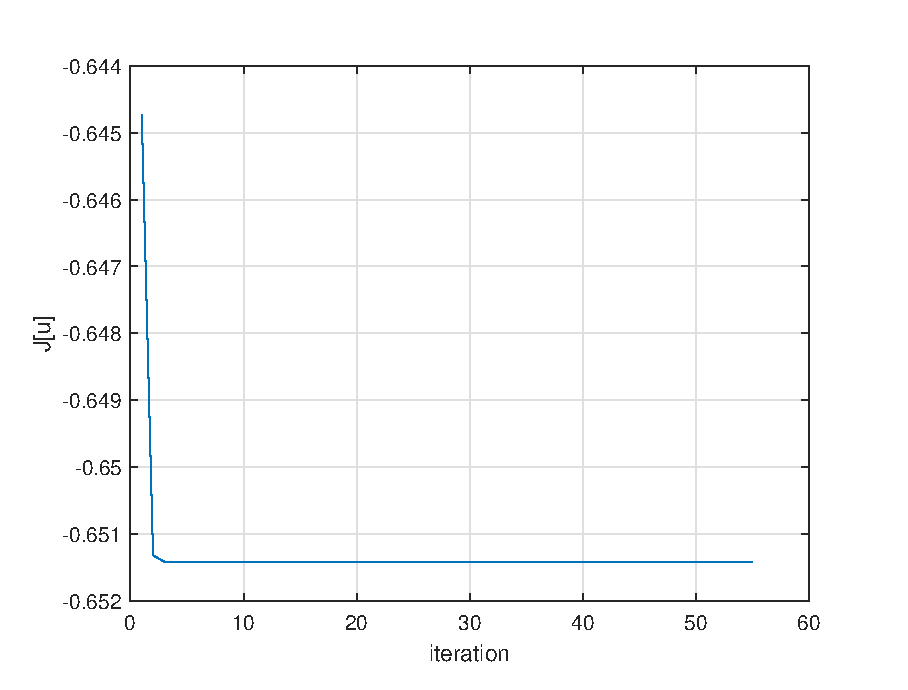
\includegraphics[width=\linewidth]{includefiles/1D p-Laplace LDG2/p=10, k=3, N=64, wei, J.eps}
			\end{center}
		\end{subfigure}
		\begin{subfigure}{0.49\linewidth}
			\begin{center}
				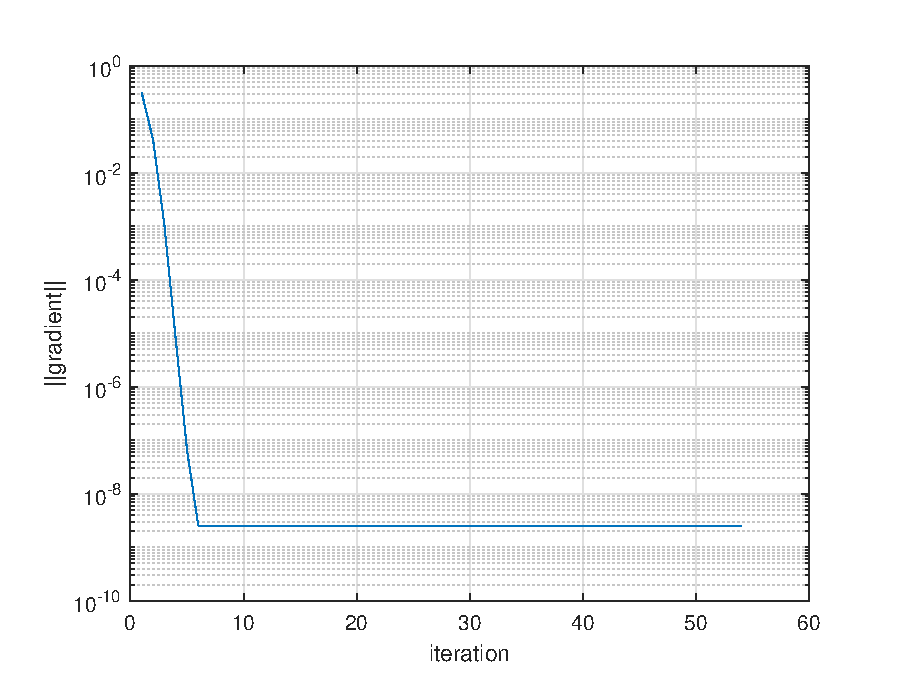
\includegraphics[width=\linewidth]{includefiles/1D p-Laplace LDG2/p=10, k=3, N=64, wei, grad.eps}
			\end{center}
		\end{subfigure}
        \begin{subfigure}{0.49\linewidth}
			\begin{center}
				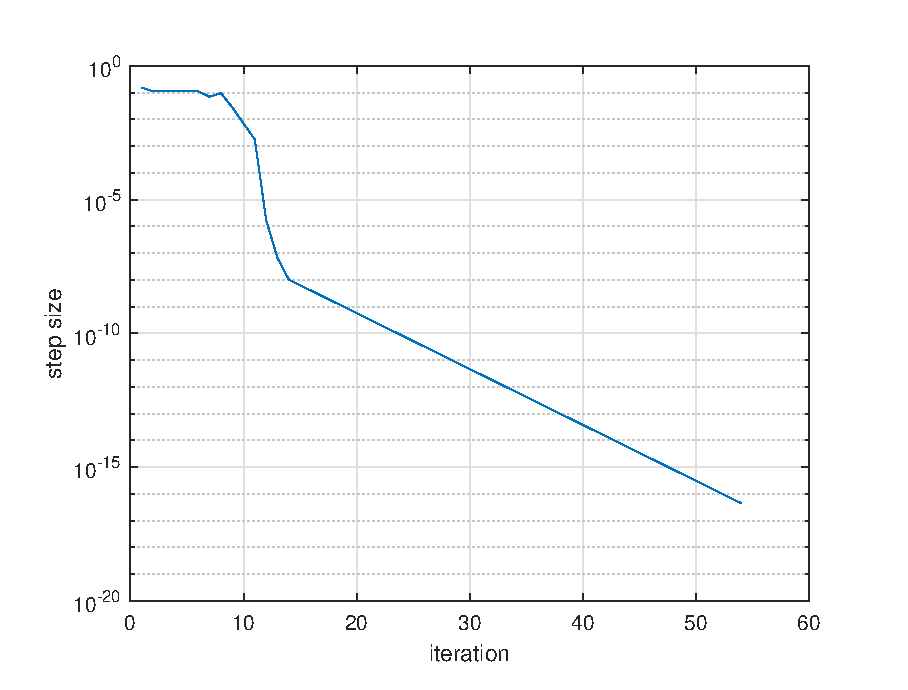
\includegraphics[width=\linewidth]{includefiles/1D p-Laplace LDG2/p=10, k=3, N=64, wei, rho.eps}
			\end{center}
		\end{subfigure}

        \caption{\(p = 10\)，\(k = 3\)，\(N = 64\)，加权预处理子}
	\end{center}
\end{figure}

\begin{figure}[H]
	\begin{center}
		\begin{subfigure}{0.49\linewidth}
			\begin{center}
				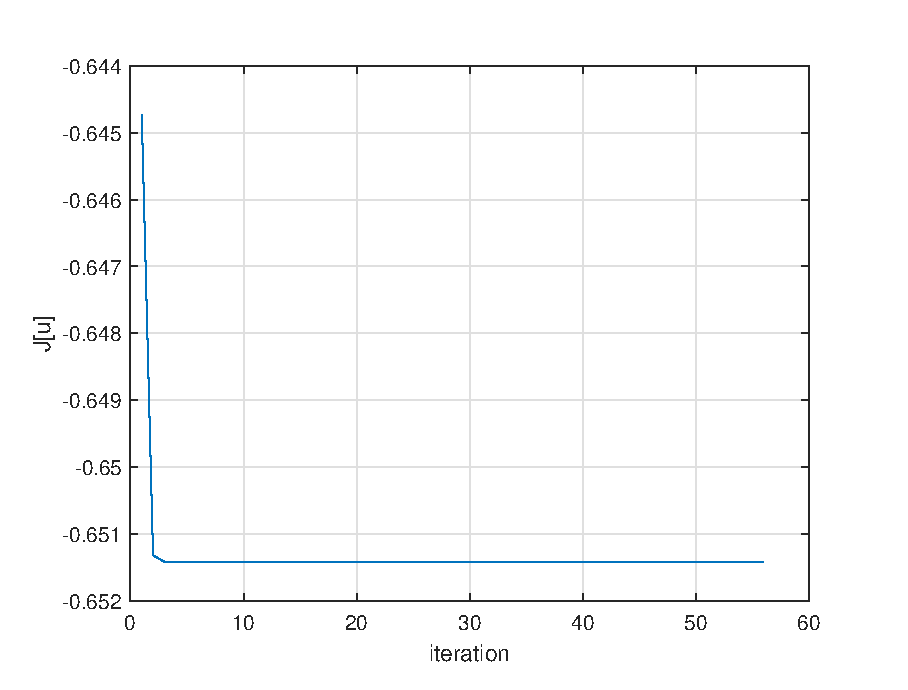
\includegraphics[width=\linewidth]{includefiles/1D p-Laplace LDG2/p=10, k=3, N=256, wei, J.eps}
			\end{center}
		\end{subfigure}
		\begin{subfigure}{0.49\linewidth}
			\begin{center}
				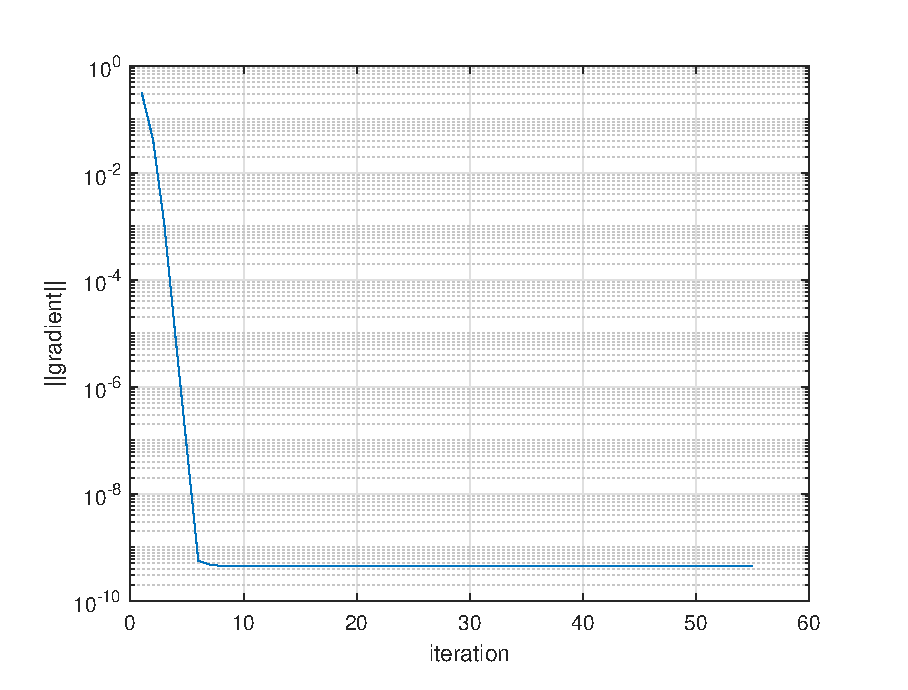
\includegraphics[width=\linewidth]{includefiles/1D p-Laplace LDG2/p=10, k=3, N=256, wei, grad.eps}
			\end{center}
		\end{subfigure}
        \begin{subfigure}{0.49\linewidth}
			\begin{center}
				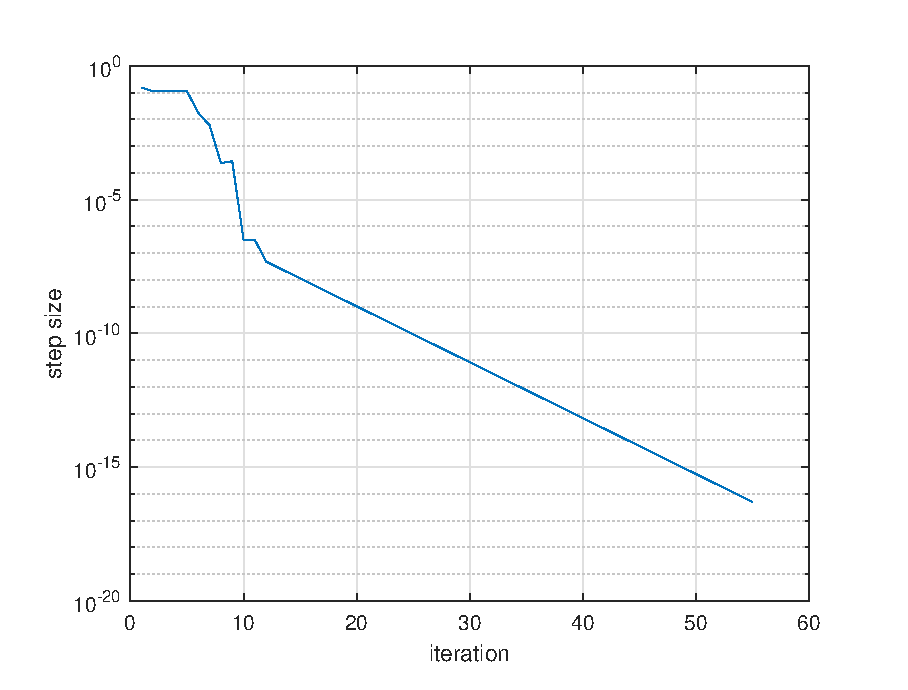
\includegraphics[width=\linewidth]{includefiles/1D p-Laplace LDG2/p=10, k=3, N=256, wei, rho.eps}
			\end{center}
		\end{subfigure}

        \caption{\(p = 10\)，\(k = 3\)，\(N = 256\)，加权预处理子}
	\end{center}
\end{figure}

\begin{figure}[H]
	\begin{center}
		\begin{subfigure}{0.49\linewidth}
			\begin{center}
				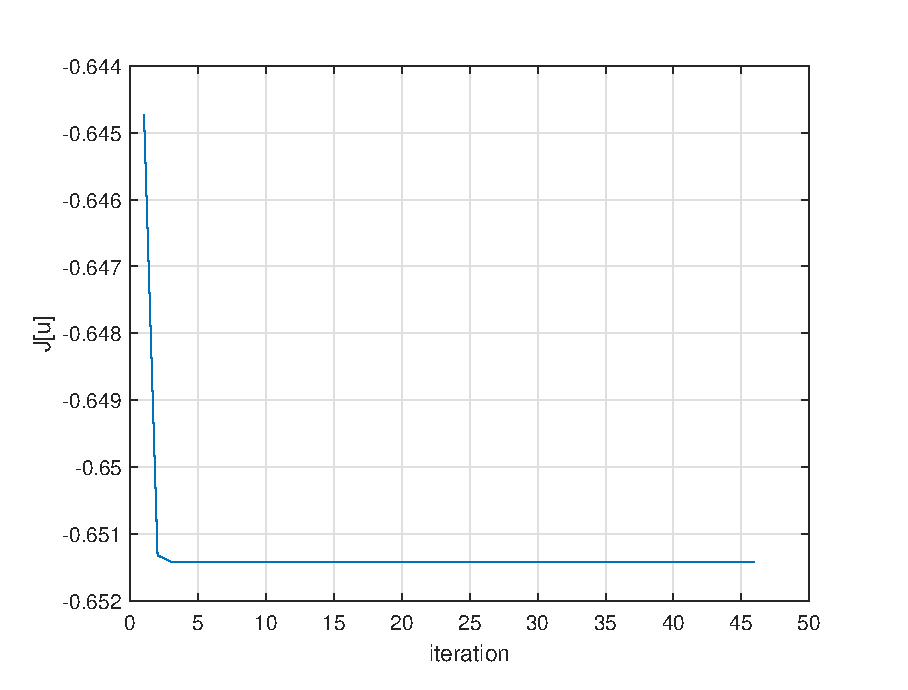
\includegraphics[width=\linewidth]{includefiles/1D p-Laplace LDG2/p=10, k=4, N=64, wei, J.eps}
			\end{center}
		\end{subfigure}
		\begin{subfigure}{0.49\linewidth}
			\begin{center}
				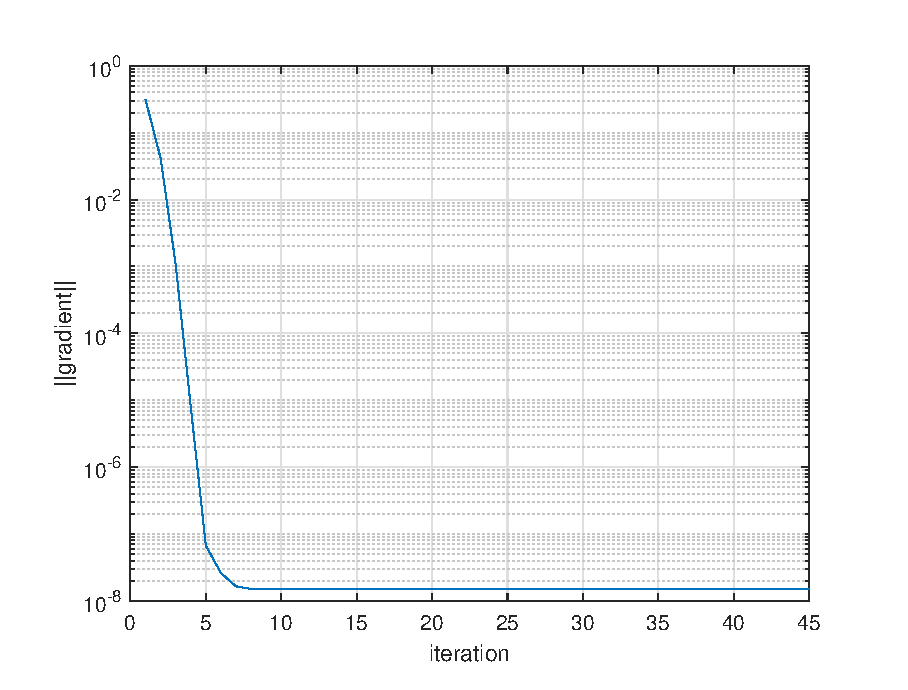
\includegraphics[width=\linewidth]{includefiles/1D p-Laplace LDG2/p=10, k=4, N=64, wei, grad.eps}
			\end{center}
		\end{subfigure}
        \begin{subfigure}{0.49\linewidth}
			\begin{center}
				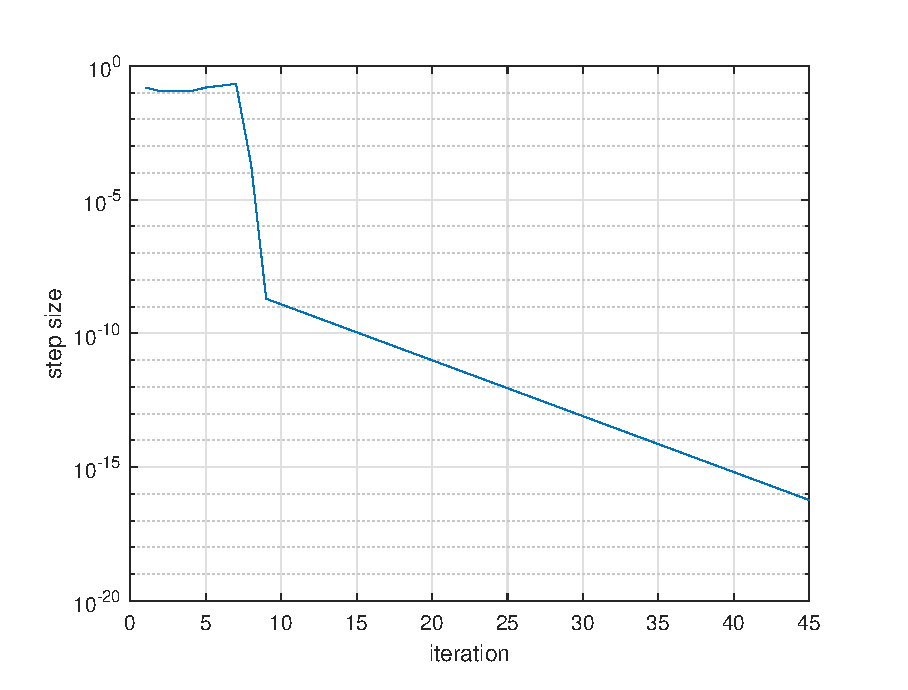
\includegraphics[width=\linewidth]{includefiles/1D p-Laplace LDG2/p=10, k=4, N=64, wei, rho.eps}
			\end{center}
		\end{subfigure}

        \caption{\(p = 10\)，\(k = 4\)，\(N = 64\)，加权预处理子}
	\end{center}
\end{figure}



测试中，所有的三种预条件子都显示出了与网格、多项式次数均无关的迭代次数和下降曲线，符合我们的预期。其中，加权预条件子的收敛速度优于 Poisson 预处理子，并显著优于标准预条件子，速度之间的差距随着 \(p + \frac{1}{p-1}\) 增大而迅速增大。在测试收敛阶时，当 \(p > 2\) 且 \(k \geqslant 2\) 时，只有加权预条件子可以给出满意的结果；Poisson 预条件子可以得到最优的 \(\sigma_{h}\) 的收敛阶，但是 \(u_{h}\) 的收敛阶则会较低。有趣的是，当 \(p > 2\) 且 \(k = 1\) 时，Poisson 预条件子和加权预条件子给出的 \(\sigma_{h}\) 的误差几乎相等，但是加权预条件子给出的 \(u_{h}\) 误差明显高于 Poisson 预条件子，经过实验我们发现 \(u_{h}\) 的误差和稳定项 \(\epsilon\) 的取值有关。除这两个预条件子之外，标准预条件子需要的迭代次数显著高于其他两者，因此我们没有采用。

在上面的算例中(以及其他收敛的 \(p\) 值测试中)，我们观察到对 \(\left(\sigma, u\right)\) 的 \(L^{p^{\ast}}\times L^{p}\) 的 \(\left(k, k+1\right)\) 阶收敛，这在 LDG 框架下是最优的。同时，当 \(p > 2\) 时，对 \(u\) 的 \(L^2\) 收敛阶比 \(L^{p}\) 收敛阶高，对 \(\sigma\) 的 \(L^2\) 收敛阶比 \(L^{p^{\ast}}\) 收敛阶低；当 \(p < 2\) 时反之。这与多项式逼近的反向估计结果一致。


\subsubsection{Conclusion}

我们的第而个 \(p\)-Laplace 方程 LDG 算法相当于用 LDG 方法直接离散最优化形式\eqref{p-Laplace primal minimization form}，而不引入中间变量。我们针对此方法，把文章\cite{10.1007/s10915-007-9134-z}中的预处理器推广到了 LDG 框架下。此方法的优势在于：
\begin{itemize}
    \item 基于梯度下降的数值格式对任何迭代初值都保证收敛，且收敛性能与网格无关。
    \item 未知函数数量少。
    \item 在数值实验中，对 \(\left(\sigma, u\right)\) 的 \(L^{p^{\ast}} \times L^{p}\) 误差有 \(\left(k, k+1\right)\) 阶收敛阶。
\end{itemize}
此方法的劣势在于：
\begin{itemize}
    \item 基于梯度下降的方法需要有效的预处理器，经过实验我们发现加权预条件子是三种预条件子里性能最好的，但是该预条件子需要加入稳定项 \(\epsilon\)，该稳定项对 \(u_{h}\) 的误差会产生的影响不可忽视。
    \item 实验其他的预条件子时，例如 Poisson 预条件子，误差可以迅速下降，但是由于浮点误差或者其他因素，数值解暂时收敛不到准确解。
\end{itemize}